\documentclass[lang=cn,10pt]{elegantbook}
\usepackage[toc]{glossaries}
\makeglossaries
\loadglsentries{glossaries}

\newcommand\citeauthoryear[1]{\citeauthor{#1}[\citeyear{#1}]}
\renewcommand{\lstlistingname}{程序}
\DeclareCiteCommand{\citeauthor}
  {\boolfalse{citetracker}%
   \boolfalse{pagetracker}%
   \usebibmacro{prenote}}
  {\ifciteindex
     {\indexnames{labelname}}
     {}%
   \printtext[bibhyperref]{\printnames{labelname}}}
  {\multicitedelim}
  {\usebibmacro{postnote}}

\title{编译原理及实践}
\author{Kenneth Louden}
\bioinfo{译者}{左元}

\setcounter{tocdepth}{3}
\cover{cover.pdf}

\usepackage{array}
\newcommand{\ccr}[1]{\makecell{{\color{#1}\rule{1cm}{1cm}}}}

\definecolor{codegreen}{rgb}{0,0.6,0}
\definecolor{codegray}{rgb}{0.5,0.5,0.5}
\definecolor{codepurple}{rgb}{0.58,0,0.82}
\definecolor{backcolour}{rgb}{0.95,0.95,0.92}

\lstdefinestyle{mystyle}{
    backgroundcolor=\color{backcolour},   
    commentstyle=\color{codegreen},
    keywordstyle=\color{magenta},
    numberstyle=\tiny\color{codegray},
    stringstyle=\color{codepurple},
    basicstyle=\ttfamily\footnotesize,
    breakatwhitespace=false,         
    breaklines=true,                 
    captionpos=b,                    
    keepspaces=true,                 
    numbers=left,                    
    numbersep=5pt,                  
    showspaces=false,                
    showstringspaces=false,
    showtabs=false,                  
    tabsize=2
}

\lstset{style=mystyle}

\begin{document}

\maketitle
\frontmatter

\tableofcontents

\mainmatter

\chapter{概论}
\label{chap:1}

\begin{introduction}
  \item 为什么要用编译器
  \item 与编译器相关的程序
  \item 翻译步骤
  \item 编译器中的主要数据结构
  \item 编译器结构中的其他问题
  \item 自举与移植
  \item TINY示例语言与编译器
  \item C-Minus:编译器项目的一种语言
\end{introduction}

编译器是将一种语言翻译为另一种语言的计算机程序。编译器将\textbf{源语言}(source language)编写的程序作为输入,而产生用\textbf{目标语言}(target language)编写的等价程序。通常地,源语言为\textbf{高级语言}(high-level language),如C或C++,而目标语言则是目标机器的目标代码(object code,有时也称作机器代码(machine code)),也就是写在计算机机器指令中的用于运行的代码。这一过程可以用下图表示:

\begin{center}
  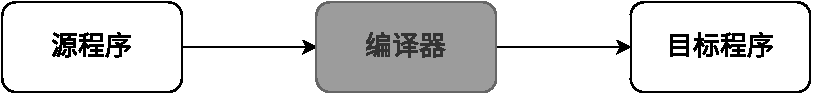
\includegraphics[width=.8\textwidth]{1.pdf}
\end{center}

编译器是一种相当复杂的程序,其代码的长度可从10000行到1000000行不等。编写甚至读懂这样的一个程序都非易事,大多数的计算机科学家和专业人员也从来没有编写过一个完整的编译器。但是,几乎所有形式的计算均要用到编译器,而且任何一个与计算机打交道的专业人员都应掌握编译器的基本结构和操作。除此之外,计算机应用程序中经常遇到的一个任务就是命令解释程序和界面程序的开发,这比编译器要小,但使用的却是相同的技术。因此,掌握这一技术具有非常大的实际意义。

也正因为这一点,本书不仅仅要讲解基础知识,还为读者提供了所有必要的工具和设计编写真正的编译器的实践。要做到这些,就必须学习各项理论知识,而这主要应从自动机原理(它使编译器结构合理)着手。在讲述时我们假设读者并不了解自动机原理。当然,此处的观点与标准的自动机原理论著有所不同,这些论著特别强调编译过程;但是,学过自动机原理的读者就会发现对这些理论材料很熟悉,这部分阅读起来也十分迅速。特别是对于那些十分了解自动机原理背景的读者来说,对\ref{sec:2-2}节、\ref{sec:2-3}节、\ref{sec:2-4}节和\ref{sec:3-2}节就不必细读了。无论怎样,读者都应知道基本的数据结构和离散数学。机器结构和汇编语言的相关知识也很重要,在第8章“代码生成”中尤为如此。

实际编码技术的研究本身就要求认真规划,这是因为即使有很好的理论基础,编码的细节也可能会复杂得令人不知如何操作。本书包括了有关程序设计语言结构的一系列简单示例,并利用它们针对该项技术进行详细描述,讨论中使用到的语言被称作TINY。此外,附录\ref{append:A}还提供了一个更广泛的示例,它包括了一个小小的但却非常复杂的适用于作为课程项目的C子集(称作C-Minus)。本书还有大量的练习,这其中包括简单的笔头训练、书中代码的扩展,以及更多的相关编程练习。

总之,在编译器结构和被编译的程序设计语言的设计之间存在着一个很重要的交互。在本书中,只是附带着讲解了一下语言设计问题,而是着重于程序设计语言的概念和设计问题(参见本章最后的“笔记与参考”部分)。

首先将简要地介绍编译器的历史及其存在目的与理由,以及与编译器相关的程序描述。接着讲解编译器的结构、各种翻译过程和相关的数据结构,并联系一个简单的具体示例来示范这个结构。最后,再概括地讲述一下编译器结构的其他问题,这包括自举和移植,以及本书后面用到的主要语言的描述。

\section{为什么要用编译器}
\label{sec:1-1}

在本世纪40年代,由于冯·诺伊曼在存储——程序计算机方面的先锋作用,编写一串代码或程序已成必要,这样计算机就可以执行所需的计算。开始时,这些程序都是用\textbf{机器语言}(machine language)编写的。机器语言就是表示机器实际操作的数字代码,例如:

C7 06 0000 0002

表示在IBM PC上使用的Intel 8x86处理器将数字2移至地址0000(16进制)的指令。当然,编写这样的代码是十分费时和乏味的,这种代码形式很快就被\textbf{汇编语言}(assembly language)代替了。在汇编语言中,都是以符号形式给出指令和存储地址的。例如,汇编语言指令

MOV X, 2

就与前面的机器指令等价(假设符号存储地址X是0000)。\textbf{汇编器}(assembler)将汇编语言的符号代码和存储地址翻译成与机器语言相对应的数字代码。

汇编语言大大提高了编程的速度和准确度,人们至今仍在使用着它,在编码需要极快的速度和极高的简洁程度时尤为如此。但是,汇编语言也有许多缺点:编写起来也不容易,阅读和理解很难;而且汇编语言的编写严格依赖于特定的机器,所以为一台计算机编写的代码在应用于另一台计算机时必须完全重写。很明显,发展编程技术的下一个重要步骤就是以一个更类似于数学定义或自然语言的简洁形式来编写程序的操作,它应与任何机器都无关,而且也可由一个程序翻译为可执行的代码。例如,前面的汇编语言代码可以写成一个简洁的与机器无关的形式

x = 2

起初人们担心这是不可能的,或者即使可能,目标代码也会因效率不高而没有多大用处。

在1954年至1957年期间,IBM的John Backus带领的一个研究小组对FORTRAN语言及其编译器的开发,使得上面的担忧不必要了。但是,由于当时处理中所涉及到的大多数程序设计语言的翻译并不为人所掌握,所以这个项目的成功也伴随着巨大的辛劳。

几乎与此同时,人们也在开发着第一个编译器,Noam Chomsky开始了他的自然语言结构的研究。他的发现最终使得编译器结构异常简单,甚至还带有了一些自动化。Chomsky的研究导致了根据语言\textbf{文法}(grammar,指定其结构的规则)的难易程度以及识别它们所需的算法来为语言分类。正如现在所称的——与\textbf{乔姆斯基分类结构}(Chomsky hierarchy)一样——包括了文法的4个层次: 0型、1型、2型和3型文法,且其中的每一个都是其前者的专门化。2型(或\textbf{上下文无关文法}(context-free grammar))被证明是程序设计语言中最有用的,而且今天它已代表着程序设计语言结构的标准方式。\textbf{语法分析问题}(parsing problem,用于限定上下文无关语言的识别的有效算法)的研究是在60年代和70年代,它相当完善地解决了这一问题,现在它已是编译理论的一个标准部分。本书的第\ref{chap:3}、\ref{chap:4}和\ref{chap:5}章将研究上下文无关的语言和语法分析算法。

\textbf{有限自动机}(finite automata)和正则表达式(regular expression)同上下文无关文法紧密相关,它们与乔姆斯基的3型文法相对应。对它们的研究与乔姆斯基的研究几乎同时开始,并且引出了表示程序设计语言的单词(或称为记号)的符号方式。第\ref{chap:2}章将讲述有限自动机和正则表达式。

人们接着又深化了生成有效的目标代码的方法,这就是最初的编译器,它们被一直使用至今。人们通常将其误称为优化技术(optimization technique),但因其从未真正地得到过被优化了的目标代码而仅仅改进了它的有效性,因此实际上应称作代码改进技术(code improvement technique)。第\ref{chap:8}章将讲述该技术的基础知识。

当语法分析问题变得好懂起来时,人们就在开发程序上花费了很大的功夫来研究这一部分的编译器的自动构造。这些程序最初被称为编译程序——编译器,但更确切地应称为语法分析器生成器(parser generator),这是因为它们仅仅能够自动处理编译的一部分。这些程序中最著名的是Yacc(yet another compiler-compiler),它是由Steve Johnson在1975年为Unix系统编写的,我们将在第\ref{chap:5}章中再次谈到它。类似地,有限自动机的研究也发展了另一种称为扫描器生成器(scanner generator)的工具,Lex(与Yacc同时,由Mike Lesk为Unix系统开发的)是这其中的佼佼者。读者将在第\ref{chap:2}章中学到Lex。

在70年代后期和80年代早期,大量的项目都关注于编译器其他部分的生成自动化,这其中就包括了代码生成。这些尝试并未取得多少成功,这大概是因为操作太复杂而人们又对其不甚了解,本书也就不详细谈它了。

编译器设计最近的发展包括:首先,编译器包括了更为复杂的算法的应用程序,它用于推断和/或简化程序中的信息;这又与更为复杂的程序设计语言(可允许此类分析)的发展结合在一起。其中典型的有用于函数语言编译的Hindley-Milner类型检查的统一算法。其次,编译器已越来越成为基于窗口的交互开发环境(interactive development environment,IDE)的一部分,它包括了编辑器、链接器、调试器以及项目管理程序。这样的IDE的标准并没有多少,但是已沿着这一方向对标准的窗口环境进行开发了。这一专题的研究超出了本书的范围(但是读者可以参阅下一节中有关IDE部件的内容)。读者可以参阅本章末尾的“注意与参考”中的文献内容。尽管近年来对此进行了大量的研究,但是基本的编译器设计在近20年中都没有多大的改变,而且它们正迅速地成为计算机科学课程中的中心一环。

\section{与编译器相关的程序}
\label{sec:1-2}

本节主要描述与编译器有关或专编译器一同使用的其他程序,以及那些在一个完整的语言开发环境中与编译器一同使用的程序(有一些已在前面提到过)。

\textbf{1. 解释器}(interpreter)

解释器是如同编译器的一种语言翻译程序。它与编译器的不同之处在于:它立即执行源程序而不是生成在翻译完成之后才执行的目标代码。从原理上讲,任何程序设计语言都可被解释或被编译,但是根据所使用的语言和翻译情况,很可能会选用解释器而不用编译器。例如,我们经常解释执行BASIC程序而不是去编译它。类似地,诸如LISP的函数式编程语言也常常是被解释执行的。解释器也经常用于教育和软件的开发,此处的程序很有可能被翻译若干次。而另一方面,当执行的速度是最为重要的因素时就使用编译器,这是因为被编译的目标代码比被解释的源代码要快得多,有时要快10倍或更多。但是,解释器具有许多与编译器共享的操作,而两者之间也有一些混合之处。本书后面也将会提到解释器,但重点仍是编译。

\textbf{2. 汇编器}(assembler)

汇编器是用于特定计算机上的汇编语言的翻译程序。正如前面所提到的,汇编语言是计算机的机器语言的符号形式,它极易翻译。有时,编译器会生成汇编语言以作为其目标语言,然后再由一个汇编器将它翻译成目标代码。

\textbf{3. 链接器}(linker)

编译器和汇编器都经常依赖于链接器,它将分别在不同的目标文件中编译或汇编的代码收集到一个可直接执行的文件中。在这种情况下,目标代码,即还未被链接的机器代码,与可执行的机器代码之间就有了区别。链接器还连接目标程序和用于标准库函数的代码,以及链接目标程序和由计算机的操作系统提供的资源(例如,存储分配程序及输入与输出设备)。有趣的是,链接器现在正在完成编译器最早的一个主要活动(这也是“编译”一词的用法,即通过收集不同的来源来构造)。因为链接过程对操作系统和处理器有极大的依赖性,本书也就不研究它了。我们也对不细分链接的目标代码和可执行的代码,这是因为对于编译技术而言,这个区别并不重要。

\textbf{4. 加载器}(loader)

编译器、汇编器或链接器生成的代码经常还不完全适用或不能执行,但是它们的主要存储器访问却可以在存储器的任何位置中且与一个不确定的起始位置相关。这样的代码被称为是可重定位的(relocatable),而加载器可处理所有的与指定的基地址或起始地址有关的可重定位的地址。加载器使得可执行代码更加灵活,但是加载处理通常是在后台(作为操作环境的一部分)或与连接相联合时才发生,加载器极少会是实际的独立程序。

\textbf{5. 预处理器}(preprocessor)

预处理器是在真正的翻译开始之前由编译器调用的独立程序。预处理器可以删除注释、包含其他文件以及执行宏(宏macro是一段重复文字的简短描写)替代。预处理器可由语言(如C)要求或以后作为提供额外功能(诸如为FORTRAN提供Ratfor预处理器)的附加软件。

\textbf{6. 编辑器}(editor)

编译器通常接受由任何生成标准文件(例如ASCII文件)的编辑器编写的源程序。最近,编译器已与另一个编辑器和其他程序捆绑进一个交互的开发环境——IDE中。此时,尽管编辑器仍然生成标准文件,但会转向正被讨论的程序设计语言的格式或结构。这样的编辑器称为基于结构的(structure based),且它早已包括了编译器的某些操作;因此,程序员就会在程序的编写时而不是在编译时就得知错误了。从编辑器中也可调用编译器以及与它共用的程序,这样程序员无需离开编辑器就可执行程序。

\textbf{7. 调试器}(debugger)

调试器是可在被编译了的程序中判定执行错误的程序,它也经常与编译器一起放在IDE中。运行一个带有调试器的程序与直接执行不同,这是因为调试器保存着所有的或大多数源代码信息(诸如行数、变量名和过程)。它还可以在预先指定的位置(称为断点(breakpoint))暂停执行,并提供有关已调用的函数以及变量的当前值的信息。为了执行这些函数,编译器必须为调试器提供恰当的符号信息,而这有时却相当困难,尤其是在一个要优化目标代码的编译器中。因此,调试又变成了一个编译问题,本书的内容就不涉及它了。

\textbf{8. 性能剖析工具}(profiler)

性能剖析工具是在执行中搜集目标程序行为统计的程序。程序员特别感兴趣的统计是每一个过程的调用次数和每一个过程执行时间所占的百分比。这样的统计对于帮助程序员提高程序的执行速度极为有用。有时编译器也甚至无需程序员的干涉就可利用性能剖析工具的输出来自动改进目标代码。

\textbf{9. 项目管理程序}(project manager)

现在的软件项目通常大到需要由一组程序员来完成,这时对那些由不同人员操作的文件进行整理就非常重要了,而这正是项目管理程序的任务。例如,项目管理程序应将由不同的程序员制作的文件的各个独立版本整理在一起,它还应保存一组文件的更改历史,这样就能维持一个正在开发的程序的连贯版本了(这对那些由单个程序员管理的项目也很有用)。项目管理程序的编写可与语言无关,但当其与编译器捆绑在一起时,它就可以保持有关特定的编译器和建立一个完整的可执行程序的链接程序操作的信息。在Unix系统中有两个流行的项目管理程序:sccs(source code control system)和rcs(revision control system)。

\section{翻译步骤}
\label{sec:1-3}

编译器内部包括了许多步骤或称为阶段(phase),它们执行不同的逻辑操作。将这些阶段设想为编译器中一个个单独的片断是很有用的,尽管在应用中它们是经常组合在一起的,但它们确实是作为单独的代码操作来编写的。图\ref{fig:compiler-phases}是编译器中的阶段和与以下阶段(文字表、符号表和错误处理器)或其中的一部分交互的3个辅助部件。这里只是简要地描述一下每个阶段,今后大家还会更详细地学到它们(文字表和符号表在\ref{sec:1-4}节中,错误处理器在\ref{sec:1-5}节)。

\begin{figure}[htbp]
  \centering
  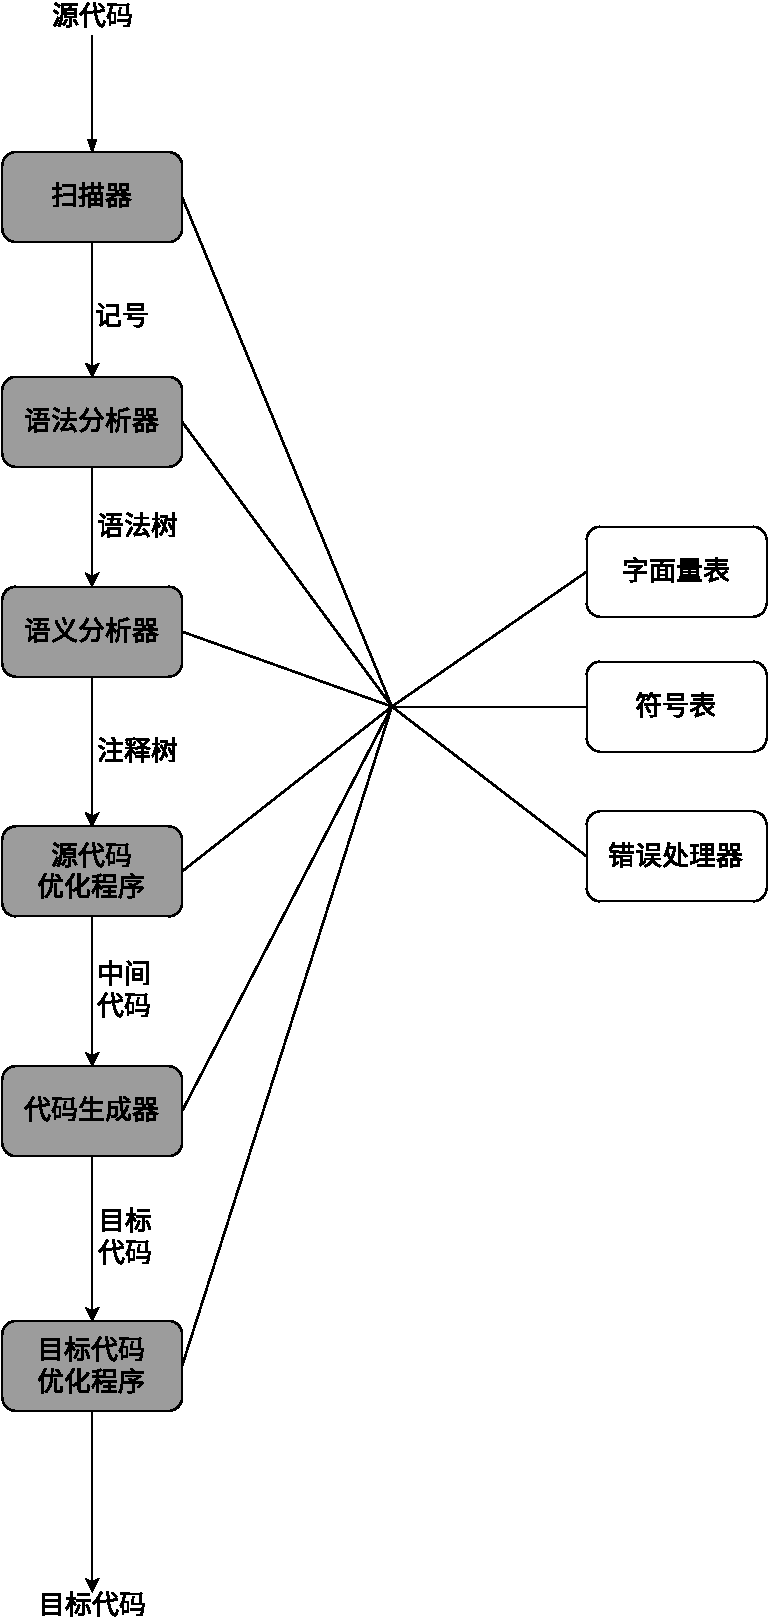
\includegraphics[width=.5\textwidth]{2.pdf}
  \caption{编译器的阶段}
  \label{fig:compiler-phases}
\end{figure}

\textbf{1. 扫描器}(scanner)

在这个阶段编译器实际阅读源程序(通常以字符流的形式表示)。扫描器执行词法分析(Lexical analysis):它将字符序列收集到称作记号(token)的有意义单元中,记号同自然语言,如英语中的字词相似。因此可以认为扫描器执行与拼写相似的任务。

例如在下面的代码行(它可以是C程序的一部分)中:

a[index] = 4 + 2

这个代码包括了12个非空字符,但只有8个记号:

\begin{tabular}{lll}
  a     & \quad\quad\quad\quad & 标识符 \\
  {[}   & \quad\quad\quad\quad & 左括号 \\
  index & \quad\quad\quad\quad & 标识符 \\
  {]}   & \quad\quad\quad\quad & 右括号 \\
  =     & \quad\quad\quad\quad & 赋值 \\
  4     & \quad\quad\quad\quad & 数字 \\
  +     & \quad\quad\quad\quad & 加号 \\
  2     & \quad\quad\quad\quad & 数字 \\
\end{tabular}

每一个记号均由一个或多个字符组成,在进一步处理之前它已被收集在一个单元中。

扫描器还可完成与识别记号一起执行的其他操作。例如,它可将标识符输入到符号表中,将字面量(literal)输入到字面量表中(字面量包括诸如3.1415926535的数字常量,以及诸如“Hello,world!”的引用字符串)。

\textbf{2. 语法分析器}(parser)

语法分析器从扫描器中获取记号形式的源代码,并完成定义程序结构的语法分析(syntax analysis),这与自然语言中句子的语法分析类似。语法分析定义了程序的结构元素及其关系。通常将语法分析的结果表示为分析树(parse tree)或语法树(syntax tree)。

例如,还是那行C代码,它表示一个称为表达式的结构元素,该表达式是一个由左边为下标表达式、右边为整型表达式的赋值表达式组成。这个结构可按下面的形式表示为一个分析树:

\begin{center}
  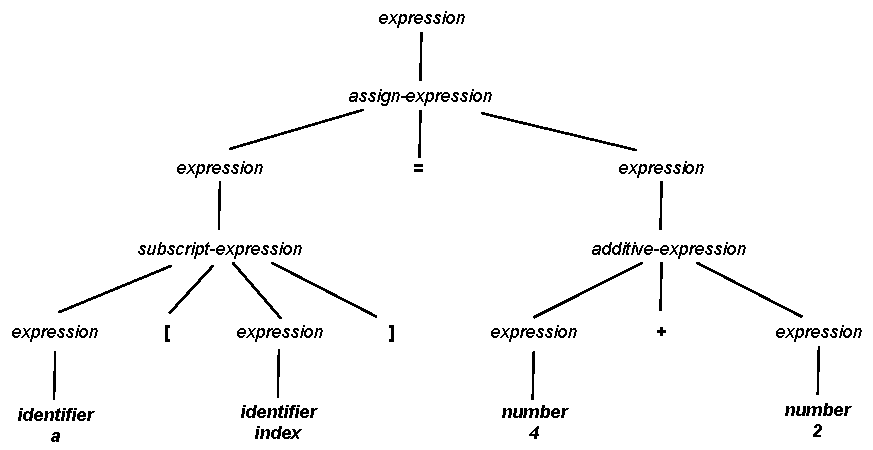
\includegraphics[width=.8\textwidth]{3.pdf}
\end{center}

请注意,分析树的内部节点均由其表示的结构名标示出,而分析树的叶子则表示输入中的记号序列(结构名以不同字体表示以示与记号的区别)。

分析树对于显示程序的语法或程序元素很有帮助,但是对于表示该结构却显得力不从心了。语法分析器更趋向于生成语法树,语法树是分析树中所含信息的浓缩(有时因为语法树表示从分析树中的进一步抽取,所以也被称为抽象语法树(abstract syntax tree))。下面是一个C赋值语句的抽象语法树的例子:

\begin{center}
  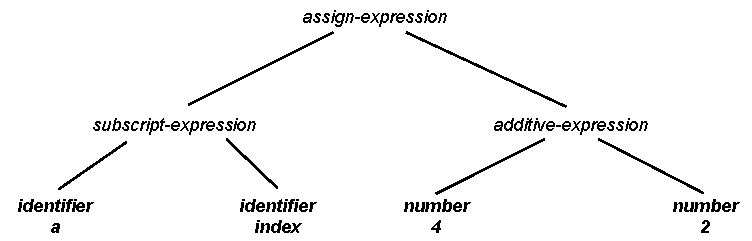
\includegraphics[width=.8\textwidth]{4.pdf}
\end{center}

请注意,在语法树中,许多节点(包括记号节点在内)已经消失。例如,如果知道表达式是一个下标运算,则不再需要用括号“[”和“]”来表示该操作是在原始输入中。

\textbf{3. 语义分析器}(semantic analyzer)

程序的语义就是它的“意思”,它与语法或结构不同。程序的语义确定程序的运行,但是大多数的程序设计语言都具有在执行之前被确定而不易由语法表示和由分析程序分析的特征。这些特征被称作静态语义(static semantic),而语义分析器的任务就是分析这样的语义(程序的“动态”语义具有只有在程序执行时才能确定的特性,由于编译器不能执行程序,所以它不能由编译器来确定)。一般的程序设计语言的典型静态语义包括声明和类型检查。由语义分析器计算的额外信息(诸如数据类型)被称为属性(attribute),它们通常是作为注释或“装饰”增加到树中(还可将属性添加到符号表中)。

在正运行的C表达式

a[index] = 4 + 2

中,该行分析之前收集的典型类型信息可能是:a是一个整型值的数组,它带有来自整型子范围的下标;index则是一个整型变量。接着,语义分析器将用所有的子表达式类型来标注语法树,并检查赋值是否使这些类型有意义了,如若没有,则声明一个类型匹配错误。在上例中,所有的类型均有意义,有关语法树的语义分析结果可用以下注释了的树来表示:

\begin{center}
  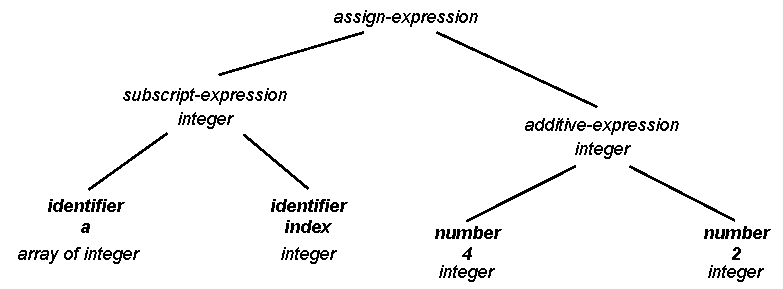
\includegraphics[width=.8\textwidth]{5.pdf}
\end{center}

\textbf{4. 源代码优化器}(source code optimizer)

编译器通常包括许多代码改进或优化步骤。绝大多数最早的优化步骤是在语义分析之后完成的,而此时代码改进可能只依赖于源代码。这种可能性是通过将这一操作提供为编译过程中的单独阶段指出的。每个编译器不论在已完成的优化种类方面还是在优化阶段的定位中都有很大的差异。

在上例中,我们包括了一个源代码层次的优化机会,也就是:表达式4 + 2可由编译器计算先得到结果6(这种优化称为常量折叠(constant folding))。当然,还会有更复杂的情况(有些将在第\ref{chap:8}章中提到)。还是在上例中,通过将根节点右面的子树合并为它的常量值,这个优化就可以直接在(注释)语法树上完成:

\begin{center}
  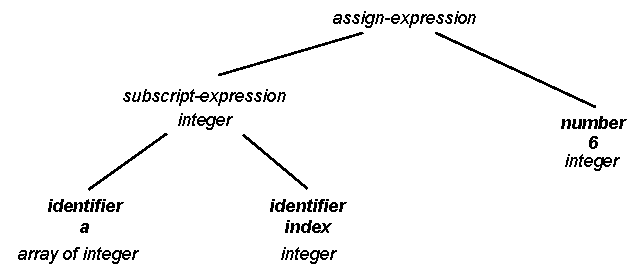
\includegraphics[width=.8\textwidth]{6.pdf}
\end{center}

尽管许多优化可以直接在树上完成,但是在很多情况下,优化接近于汇编代码线性化形式的树更为简便。这样节点的变形有许多,但是三地址码(three-address code)(之所以这样称呼是因为它在存储器中包含了3个(或3个以上)位置的地址)却是标准选择。另一个常见的选择是p-code,它常用于Pascal编译器中。

在前面的例子中,原先的C表达式的三地址码应是:

\begin{lstlisting}
  t = 4 + 2
  a[index] = t
\end{lstlisting}

(请注意,这里利用了一个额外的临时变量t存放加法的中间值)。这样,优化程序就将这个代码改进为两步。首先计算加法的结果:

\begin{lstlisting}
  t = 6
  a[index] = t
\end{lstlisting}

接着,将t替换为该值以得到三地址码

a[index] = 6

图\ref{fig:compiler-phases}已经指出源代码优化器可能通过将其输出称为中间代码(intermediate code)来使用三地址码。中间代码一直是指一种位于源代码和目标代码(例如三地址码或类似的线性表示)之间的代码表示形式。但是,我们可以更概括地认为它是编译器使用的源代码的任何一个内部表示。此时,也可将语法树称作中间代码,源代码优化器则确实能继续在其输出中使用这个表示。有时,这个中间代码也称作中间表示(intermediate representation, IR)。

\textbf{5. 代码生成器}

代码生成器得到中间代码(IR),并生成目标机器的代码。尽管大多数编译器直接生成目标代码,但是为了便于理解,本书用汇编语言来编写目标代码。正是在编译的这个阶段中,目标机器的特性成为了主要因素。当它存在于目标机器时,使用指令不仅是必须的而且数据的形式表示也起着重要的作用。例如,整型数据类型的变量和浮点数据类型的变量在存储器中所占的字节数或字数也很重要。

在上面的示例中,现在必须决定怎样存储整型数来为数组索引生成代码。例如,下面是所给表达式的一个可能的样本代码序列(在假设的汇编语言中):

\begin{lstlisting}
  MOV         R0, index     ;; value of index -> R0
  MUL         R0, 2         ;; double value in R0
  MOV         R1, &a        ;; address of a -> R1
  ADD         R1, R0        ;; add R0 to R1
  MOV         *R1, 6        ;; constant 6 -> address in R1
\end{lstlisting}

在以上代码中,为编址模式使用了一个类似C的协定,因此\&a是a的地址(也就是数组的基地址),*R1则意味着间接寄存器地址(因此最后一条指令将值6存放在R1包含的地址中)。这个代码还假设机器执行字节编址,并且整型数占据存储器的两个字节(所以在第2条指令中用2作为乘数)。

\textbf{目标代码优化器}(target code optimizer)

在这个阶段中,编译器尝试着改进由代码生成器生成的目标代码。这种改进包括选择编址模式以提高性能、将速度慢的指令更换成速度快的,以及删除多余的操作。

在上面给出的样本目标代码中,还可以做许多更改:在第2条指令中,利用移位指令替代乘法(通常地,乘法很费时间),还可以使用更有效的编址模式(例如用索引地址来执行数组存储)。使用了这两种优化后,目标代码就变成:

\begin{lstlisting}
  MOV         R0, index      ;; value of index -> R0
  SHL         R0             ;; double value in R0
  MOV         &a[R0], 6      ;; constant 6 -> address a + R0
\end{lstlisting}

到这里,对编译器阶段的简要描述就结束了,但我们还应特别强调这些讲述仅仅是示意性的,也无需表示出正在工作中的编译器的实际结构。编译器在其结构细节上确实差别很大,然而,上面讲到的阶段总会出现在几乎所有的编译器的某个形式上。

我们还谈到了用于维持每一个阶段所需信息的数据结构,例如语法树、中间代码(假设它们并不相同)、文字表和符号表。下一节是编译器中的主要数据结构的概览。

\section{编译器中的主要数据结构}
\label{sec:1-4}

当然,由编译器的阶段使用的算法与支持这些阶段的数据结构之间的交互是非常强大的。编译器的编写者尽可能有效实施这些方法且不引起复杂性。理想的情况是:与程序大小成线性比例的时间内编译器,换言之就是,在O(n)时间内,n是程序大小的度量(通常是字符数)。本节将讲述一些主要的数据结构,它们是其操作部分阶段所需要的,并用来在阶段中交流信息。

\textbf{1. 记号}(token)

当扫描器将字符收集到一个记号中时,它通常是以符号表示这个记号;这也就是说,作为一个枚举数据类型的值来表示源程序的记号集。有时还必须保留字符串本身或由此派生出的其他信息(例如:与标识符记号相关的名字或数字记号值)。在大多数语言中,扫描器一次只需要生成一个记号(这称为单符号先行(single symbol lookahead))。在这种情况下,可以用全局变量放置记号信息;而在别的情况(最为明显的是FORTRAN)下,则可能会需要一个记号数组。

\textbf{2. 语法树}(syntax tree)

如果分析程序确实生成了语法树,它的构造通常为基于指针的标准结构,在进行分析时动态分配该结构,则整棵树可作为一个指向根节点的单个变量保存。结构中的每一个节点都是一个记录,它的域表示由分析程序和之后的语义分析器收集的信息。例如,一个表达式的数据类型可作为表达式的语法树节点中的域。有时为了节省空间,这些域也是动态分配或存放在诸如符号表的其他数据结构中,这样就可以有选择地进行分配和释放。实际上,根据它所表示的语言结构的类型(例如:表达式节点对于语句节点或声明节点都有不同的要求),每一个语法树节点本身都可能要求存储不同的属性。在这种情况下,可由不同的记录表示语法树中的每个节点,每个节点类型只包含与本身相关的信息。

\textbf{3. 符号表}(symbol table)

这个数据结构中的信息与标识符有关:函数、变量、常量以及数据类型。符号表几乎与编译器的所有阶段交互:扫描器、分析程序或将标识符输入到表格中的语义分析器;语义分析器将增加数据类型和其他信息;优化阶段和代码生成阶段也将利用由符号表提供的信息选出恰当的代码。因为对符号表的访问如此频繁,所以插入、删除和访问操作都必须比常规操作更有效。尽管可以使用各种树的结构,但杂凑表却是达到这一要求的标准数据结构。有时在一个列表或栈中可使用若干个表格。

\textbf{4. 字面量表}(literal table)

字面量表的功能是存放在程序中用到的常量和字符串,因此快速插入和查找在字面量表中也十分重要。但是,在其中却无需删除,这是因为它的数据全程应用于程序而且常量或字符串在该表中只出现一次。通过允许重复使用常量和字符串,字面量表对于缩小程序在存储器中的大小显得非常重要。在代码生成器中也需要字面量表来构造用于常数和在目标代码文件中输入数据定义的符号地址。

\textbf{5. 中间代码}(intermediate code)

根据中间代码的类型(例如三地址码和p-code)和优化的类型,该代码可以是文本串的数组、临时文本文件或是结构的连接列表。对于进行复杂优化的编译器,应特别注意选择允许简单重组的表示。

\textbf{6. 临时文件}(temporary file)

计算机过去一直未能在编译器时将整个程序保留在存储器中。这一问题已经通过使用临时文件来保存翻译时中间步骤的结果或通过“匆忙地”编译(也就是只保留源程序早期部分的足够信息用以处理翻译)解决了。存储器的限制现在也只是一个小问题了,现在可以将整个编译单元放在存储器之中,特别是在可以分别编译的语言中时。但是偶尔还是会发现需要在某些运行步骤中生成中间文件。其中典型的是代码生成时需要反填(backpatch)地址。例如,当翻译如下的条件语句时

if x = 0 then ... else ...

在知道else部分代码的位置之前必须由文本跳到else部分:

\begin{lstlisting}
  CMP X, 0
  JNE NEXT ;; location of NEXT not yet known
  <code for then-part>
  NEXT:
  <code for else-part>
\end{lstlisting}

通常,必须为NEXT的值留出一个空格,一旦知道该值后就会将该空格填上,利用临时文件可以很容易地做到这一点。

\section{编译器结构中的其他问题}
\label{sec:1-5}

可从许多不同的角度来观察编译器的结构。\ref{sec:1-3}节已讲述了它的阶段——用来表示编译器的逻辑结构。此外,还有其他一些可能的观点:编译器的物理结构、操作的顺序等等。由于编译器的结构对其可靠性、有效性、可用性以及可维护性都有很大的影响,所以编译器的编写者应熟悉尽可能多的有关编译器结构的观点。本节将考虑编译器结构的其他方面以及每一个观点是如何应用的。

\begin{center}
  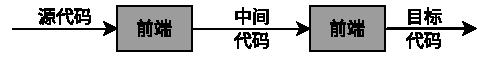
\includegraphics[width=.8\textwidth]{7.pdf}
\end{center}

\textbf{1. 分析和综合}

在这个观点中,已将分析源程序以计算其特性的编译器操作归为编译器的分析(analysis)部分,而将生成翻译代码时所涉及到的操作称作编译器的综合(synthesis)部分。当然,词法分析、语法分析和语义分析均属于分析部分,而代码生成却是综合部分。在优化步骤中,分析和综合都有。分析正趋向于易懂和更具有数学性,而综合则要求更深的专业技术。因此,将分析步骤和综合步骤两者区分开来以便发生变化时互不影响是很有用的。

\textbf{2. 前端和后端}

本观点认为,将编译器分成了只依赖于源语言(前端(front end))的操作和只依赖于目标语言(后端(back end))的操作两部分。这与将其分成分析和综合两部分是类似的:扫描器、分析程序和语义分析器是前端,代码生成器是后端。但是一些优化分析可以依赖于目标语言,这样就是属于后端了,然而中间代码的综合却经常与目标语言无关,因此也就属于前端了。在理想情况下,编译器被严格地分成这两部分,而中间表示则作为其间的交流媒介。

这一结构对于编译器的可移植性(portability)十分重要,此时设计的编译器既能改变源代码(它涉及到重写前端),又能改变目标代码(它还涉及到重写后端)。在实际中,这是很难做到的,而且称作可移植的编译器仍旧依赖于源语言和目标语言。其部分原因是程序设计语言和机器构造的快速发展以及根本性的变化,但是有效地保持移植一个新的目标语言所需的信息或使数据结构普遍地适合改变为一个新的源语言所需的信息却十分困难。然而人们不断分离前端和后端的努力会带来更方便的可移植性。

\textbf{3. 趟}

编译器发现,在生成代码之前多次处理整个源程序很方便。这些重复就是趟(pass)。第一趟是从源中构造一个语法树或中间代码,在它之后的趟是由处理中间表示、向它增加信息、更换结构或生成不同的表示组成。趟可以和阶段相应,也可无关——趟中通常含有若干个阶段。实际上,根据语言的不同,编译器可以是一趟(one pass)——所有的阶段由一趟完成,其结果是编译得很好,但(通常)代码却不太有效。Pascal语言和C语言均允许单趟编译。(Modula-2语言的结构则要求编译器至少有两趟)。大多数带有优化的编译器都需要超过一趟:典型的安排是将一趟用于扫描和分析,将另一趟用于语义分析和源代码层优化,第3趟用于代码生成和目标层的优化。更深层的优化则可能需要更多的遍:5趟、6趟、甚至8趟都是可能的。

\textbf{4. 语言定义和编译器}

我们注意到在\ref{sec:1-1}节中,程序设计语言的词法和语法结构通常用形式的术语指定,并使用正则表达式和上下文无关文法。但是,程序设计语言的语义通常仍然是由英语(或其他的自然语言)描述的。这些描述(与形式的词法及语法结构一起)一般是集中在一个语言参考手册(language reference manual)或语言定义(language definition)之中。因为编译器的编写者掌握的技术对于语言的定义有很大的影响,所以在使用了一种新的语言之后,语言的定义和编译器同时也能够得到开发。类似地,一种语言的定义对于构造编译器所需的技术也有很大的关系。

编译器的编写者更经常遇到的情况是:正在实现的语言是众所周知的并已有了语言定义。有时这个语言定义已达到了某个语言标准(language standard)的层次,语言标准是指得到诸如美国国家标准协会(American National Standards Institute,ANSI)或国际标准化组织(International Organization for Standardization,ISO)的官方标准组织批准的标准。FORTRAN、Pascal和C语言就具有ANSI标准,Ada有一个通过了美国政府批准的标准。在这种情况下,编译器的编写者必须解释语言的定义并执行符合语言定义的编译器。通常做到这一点并不容易,但是有时由于有了标准测试程序集(测试组(test suite)),就能够测试编译器(Ada有这样一个测试组),这又变得简单起来了。文本中使用的TINY示范语言有其词法、语法和语义结构,在\ref{sec:2-5}节、\ref{sec:3-7}节和\ref{sec:6-5}节中将分别谈到这些。附录A包括了用于C-Minus编译器项目语言的一个最小的语言参考手册。

有时候,一种语言可从数学术语的形式定义(formal definition)中得到它的语义。现在人们已经使用了许多方法,尽管一个称作表示语义(denotational semantics)的方法已经成为较为常用的方法,在函数编程共同体中尤为如此,但现在仍然没有一种可成为标准的方法。当语言有一个形式定义时,那么在理论上就有可能给出编译器与该定义一致的数学证明,但是由于这太难了而几乎从未有人做过。无论怎样,该技术已超出了本书的范围,本书也不会涉及到形式语义方面的知识。

运行时环境的结构和行为是尤其受到语言定义影响的编译器构造的一个方面。运行时环境将在第7章中学习。尽管此时它没有多大用处,但程序设计语言所允许的数据结构(尤其是被许可的函数调用和返回值的类型)对于运行时系统的复杂程度具有决定性意义。以下是运行时环境的3个基本类型(按难易程度排列):

首先是FORTRAN77,它没有指针或动态分配,也没有递归函数调用,但它允许有一个完整的静态运行时环境。在这个环境中,所有存储器的分配都在执行之前进行。因为无需生成代码来维护环境,编译器的编写者的分配工作也就容易许多了。其次是Pascal、C和其他类似Algol的语言,它们允许有限动态分配以及递归函数的调用,并且要求“半动态”或带有额外的动态结构(称为堆,由此程序员可安排动态分配)的基于栈的运行时环境。最后是面向对象的函数语言,如LISP和Smalltalk,它们要求“完全动态”的环境,在其中所有的分配都是由编译器的生成代码自动完成的。因为它要求也能够自动释放存储器,而这又相应地要求复杂的“垃圾回收”算法,所以它很复杂。在学习运行时环境时将会讨论到它,但是更为复杂的内容就超出本书的范围了。

\textbf{5. 编译器的选项和界面}

编译器结构的一个重要方面是包含了一种机制与操作系统相连接,并为了满足用户的各种目的而提供选择。界面机制的例子是提供对目标机器的文件系统的访问以及输入和输出功能。用户的选项可包括列表特征(长度、出错信息和相互对照表)的说明和代码优化选项(只是某个优化的执行)。选项和界面共称为编译器的语用学(pragmatics)。有时一种语言的定义指出必须提供的语用学。例如,Pascal和C语言均指出一定的输入/输出过程(在Pascal中,它们是语言特性中的一部分;而在C语言中,它们是标准库说明的一个部分)。在Ada中,许多编译器的指示(称为(pragmas))则是语言定义的一部分。例如:Ada语句

\begin{lstlisting}
  pragma LIST(ON);
  ...
  pragma LIST(OFF);
\end{lstlisting}

为包含在pragmas中的程序部分生成了一个编译器列表。在这个文本中,我们发现编译器指示仅存在于用作编译器调试的生成列表信息的上下文中;另外,也不会在输入/输出和操作系统界面中处理问题,这是因为它们涉及到了大量的细节,而且随操作系统的不同而有很大差异。

\textbf{6. 错误处理}

编译器的一个最为重要的功能是其对源程序中错误的反应。几乎在编译的每一个阶段中都可以诊察出错误来。这些静态(或称为编译时(compile-time))的错误(static error)必须由编译器来报告,而编译器能够生成有意义的出错信息并在每一个错误之后恢复编译是非常重要的。编译器的每一个阶段都需要一个类型略为不同的出错处理,因此错误处理器(error handler)必须包括不同的操作,每个操作都给出指定的阶段和结构。因此,读者将在相应的章节中学到每一个阶段的出错处理技术。

语言定义经常要求编译器不仅能够找到静态错误,而且还能找到执行错误。这就需要编译器生成额外的代码,该代码将执行恰当的运行时测试,以保证所有这样的错误都将在执行时引起一个合适的事件。在此类事件中,最简单的就是中止程序的执行。但这经常是不合适的,而且语言的定义可能要求存在异常处理(exception handling)机制。这将使运行时系统的管理变得非常复杂,当程序可能由错误发生处继续执行时尤其如此。本书并不涉及到这样一个机制的执行情况,但会提到编译器如何生成测试代码,以保证指定的运行时错误引起执行中止。

\section{自举与移植}
\label{sec:1-6}

前面已经讨论过源语言和目标语言在编译器结构中的决定因素,以及将源语言和目标语言分为前端和后端的作用,但是却未提到过编译器构造过程中涉及到的另一个语言:编写编译器本身使用的语言。为了使编译器能立即执行,这个执行(或宿主 (host))语言只能是机器语言。当时并没有编译器,因此这确实是最初的编译器编写所用的语言。现在更为合理的方法是用另一种语言来编写编译器,而使用该种语言的编译器早已存在了。如果现存的编译器已经在目标机器上运行了,则只需利用现存的编译器编译出新的编译器以得到可运行的程序:

\begin{center}
  
\includegraphics[width=.8\textwidth]{8.pdf}
\end{center}

当语言B的现存编译器没有运行在目标机器上时,情况会更复杂一些。编译将产生一个交叉编译器(cross compiler),也就是一个为不同于它在运行之上的机器生成目标代码的编译器。这种以及其他更为复杂的情况最好通过将编译器画成一个T型图(T-diagram)(以其形状来命名)来描述。用语言H(代表宿主语言)编写的编译器将语言S(代表源语言)翻译为语言T(代表目标语言)可画成以下的T型图:

\begin{center}
  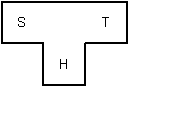
\includegraphics[width=.8\textwidth]{9.pdf}
\end{center}

请注意,这与表示编译器是在“机器”H上运行是等价的(如果H不是机器代码,则可认为其是一个假定机器的可执行代码)。我们一般都希望H与T相同(也就是编译器为与之运行之上一样的机器生成代码),但是也并不是必须这样做。

可以用两种方法组合T型图。一种是,如果在一台机器H上运行有两个编译器,其中一个编译器将语言A翻译为语言B,另一个将语言B翻译为语言C,就可按照将第1个的输出作为第2个的输入来组合。其所得结果就是一个在机器H上的由A到C的编译。将该过程表示为:

\begin{center}
  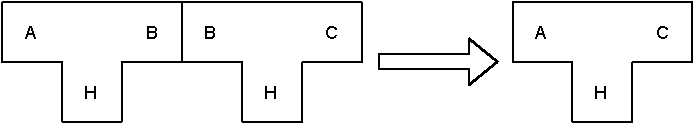
\includegraphics[width=.8\textwidth]{10.pdf}
\end{center}

另一种是,利用由“机器”H到“机器”K的编译器来翻译由H到K的其他编译器的执行语言。表示如下:

\begin{center}
  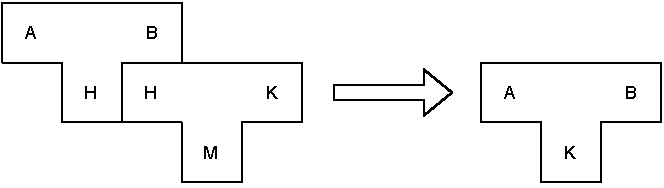
\includegraphics[width=.8\textwidth]{11.pdf}
\end{center}

在上面的描述中,第1个假定是,在机器H上利用语言B现存的编译器将语言A翻译为用B编写的语言H。它是前面所讲的特例,如下所示:

\begin{center}
  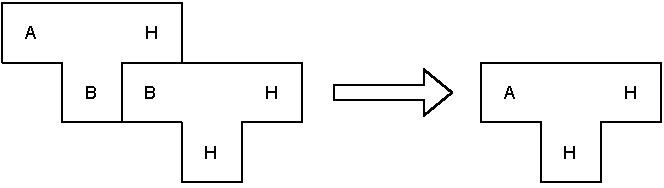
\includegraphics[width=.8\textwidth]{12.pdf}
\end{center}

第2个假定是,当语言B的编译器运行在另一台机器上时,就会引出语言A的交叉编译器。如下图所示:

\begin{center}
  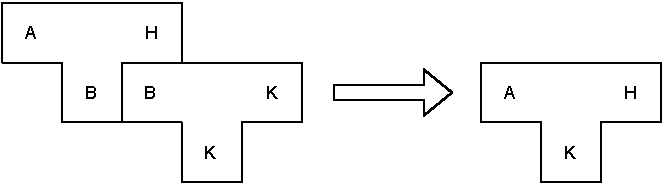
\includegraphics[width=.8\textwidth]{13.pdf}
\end{center}

以将要编译的相同语言编写一个编译器是很普通的:

\begin{center}
  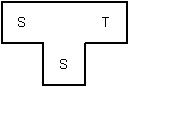
\includegraphics[width=.8\textwidth]{14.pdf}
\end{center}

但这将表现为一个循环错误:因为如果源语言的编译器不存在,那么编译器本身也就不可能被编译了。从这个方法中可以得到很重要的启示。

让我们设想一个问题:如何解决循环。我们可以在汇编语言中编写一个“虽快但不佳”的编译器,并翻译那些在编译器中真正使用得到的语言特征(当然,在编写“较好的”编译器时,会对使用那些特征有所限制)。这些“虽快但不佳”的编译器也可能产生极为无效的代码(它仅需要正确而已!)。一旦运行这个“虽快但不佳”的编译器,就可用它来编译那个“较好的”编译器。接着,对“较好的”编译器进行重编译以得到最终的版本。人们将这个过程称为自举(bootstrapping)。图\ref{fig:1-2}(a)和图\ref{fig:1-2}(b)描述了这一过程。

\begin{figure}[htbp]
  \centering
  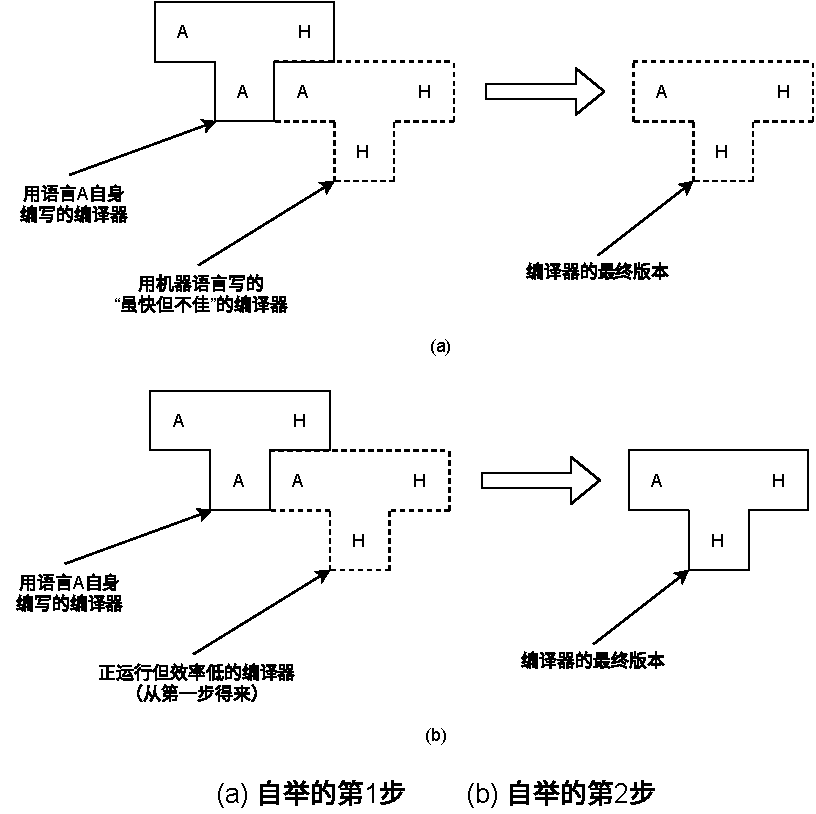
\includegraphics[width=.8\textwidth]{15.pdf}
  \caption{自举过程}
  \label{fig:1-2}
\end{figure}

自举之后,在源代码和执行代码中就有了一个编译器。这样做的好处在于:通过应用与前面相同的两步过程,编译器的源代码的任何改进都会立即被自举到一个正在工作着的编译器中。

除此之外,还有一个好处。现在将编译器移植到一个新的主机,只要求重写源代码的后端来生成新机器的代码。接着用旧的编译器来编译它以生成一个交叉编译器,该编译器又再次被交叉编译器重新编译,以得到新机器的工作版本。图\ref{fig:1-3}(a)和图\ref{fig:1-3}(b)描述了这一过程。

\begin{figure}[htbp]
  \centering
  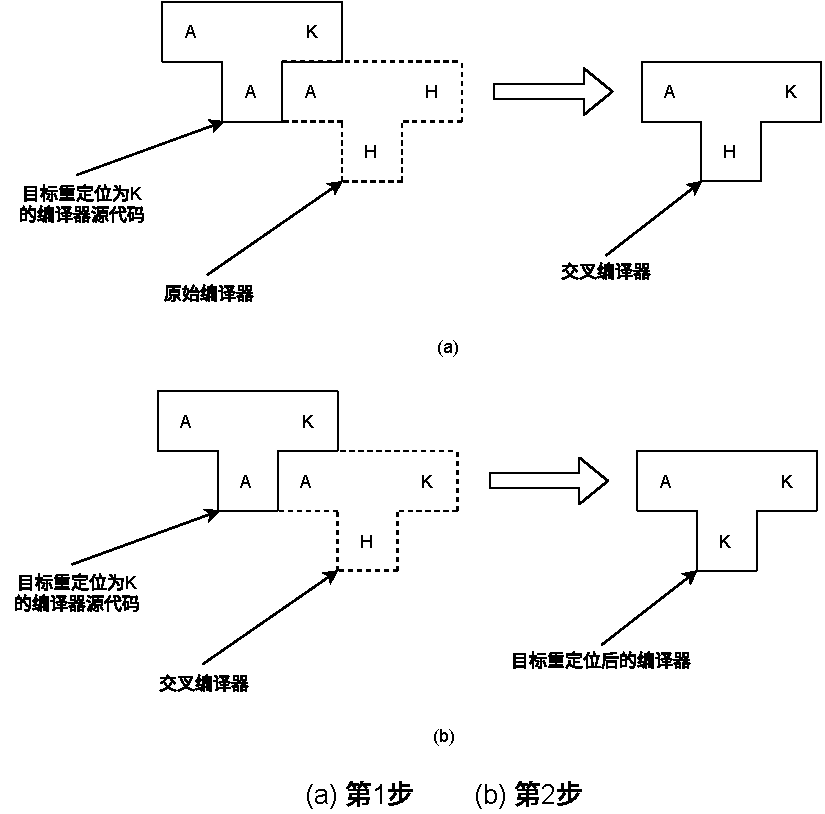
\includegraphics[width=.8\textwidth]{16.pdf}
  \caption{移植一个在其自身源代码中编写的编译器}
  \label{fig:1-3}
\end{figure}

\section{TINY示例语言与编译器}
\label{sec:1-7}

任何一本关于编译结构的书如果不包括编译过程步骤的示例就不能算完整。本书将会多次用从现有的语言(如C、C++、Pascal和Ada)中抽取的实例来讲解。但是仅用这些实例来描述编译器的各个部分是如何协调一致的却不够。因此,写出一个完整的编译器并对其操作进行注释仍是很必要的。

描述真实的编译器非常困难。“真正的”编译器——也就是希望在每天编程中用到的——内容太复杂而且不易在本教材中掌握。另一方面,一种很小的语言(其列表包括10页左右的文本)的编译也不可能准确地描述出“真正的”编译器所需的所有特征。

为了解决上述问题,人们在(ANSI)C中为小型语言提供了完整的源代码,一旦能明白这种技术,就能够很容易地理解这种小型语言的编译器了。这种语言称作TINY,在每一章的示例中都会用到它,它的编译代码也很快会被提到。完整的编译代码汇集在附录B中。

还有一个问题是:选择哪一种机器语言作为TINY编译器的目标语言?为现有的处理器使用真正的机器代码的复杂性使得这个选择很困难。但是选择特定的处理器也将影响到执行这些机器生成的目标代码。相反地,可将目标代码简化为一个假定的简单处理器的汇编语言,这个处理器称为TM机(tiny machine)。在这里只是简单地谈谈,详细内容将放在第\ref{chap:8}章(代码生成)中。附录\ref{append:C}有C的TM模拟程序列表。

\subsection{TINY语言}
\label{subsec:1-7-1}

TINY的程序结构很简单,它在语法上与Ada或Pascal的语法相似:仅是一个由分号分隔开的语句序列。另外,它既无过程也无声明。所有的变量都是整型变量,通过对其赋值可较轻易地声明变量(类似FORTRAN或BASIC)。它只有两个控制语句:if语句和repeat语句,这两个控制语句本身也可包含语句序列。If语句有一个可选的else部分且必须由关键字end结束。除此之外,read语句和write语句完成输入/输出。在花括号中可以有注释,但注释不能嵌套。

TINY的表达式也局限于布尔表达式和整型算术表达式。布尔表达式由对两个算术表达式的比较组成,该比较使用<与=比较算符。算术表达式可以包括整型常数、变量、参数以及4个整型算符+、-、*、/,此外还有一般的数学属性。布尔表达式可能只作为测试出现在控制语句中——而没有布尔型变量、赋值或I/O。

程序\ref{code:1-1}是该语言中的一个阶乘函数的简单编程示例。这个例子在整本书中都会用到。

\begin{lstlisting}[caption={一个输出其输入阶乘的TINY语言程序},label={code:1-1}]
  { Sample program
    in TINY language -
    computes factorial
  }
  read x; { input an integer }
  if x > 0 then { don't compute if x <= 0 }
    fact := 1;
    repeat
      fact := fact * x;
      x := x - 1;
    until x = 0;
    write fact { output factorial of x }
  end
\end{lstlisting}

虽然TINY缺少真正程序设计语言所需要的许多特征——过程、数组且浮点值是一些较大的省略——但它足可以用来例证编译器的主要特征了。

\subsection{TINY编译器}
\label{subsec:1-7-2}

TINY编译器包括以下的C文件,(为了包含而)把它的头文件放在左边,它的代码文件放在右边:

\begin{lstlisting}
  globals.h        main.c
  util.h           util.c
  scan.h           scan.c
  parse.h          parse.c
  symtab.h         symtab.c
  analyze.h        analyze.c
  code.h           code.c
  cgen.h           cgen.c
\end{lstlisting}

除了将main.c放在globals.h的前面之外,这些文件的源代码及其行号都按顺序列在附录B中了。任何代码文件都包含了globals.h头文件,它包括了数据类型的定义和整个编译器均使用的全局变量。main.c文件包括运行编译器的主程序,它还分配和初始化全局变量。其他的文件则包含了头/代码文件对、在头文件中给出了外部可用的函数原型以及在相关代码文件中的实现(包括静态局部函数)。scan、parse、analyze和cgen文件与图\ref{fig:compiler-phases}中的扫描器、分析程序、语义分析器和代码生成器各阶段完全相符。util文件包括了实用程序函数,生成源代码(语法树)的内部表示和显示列表与出错信息均需要这些函数。symtab文件包括执行与TINY应用相符的符号表的杂凑表。code文件包括用于依赖目标机器(将在\ref{subsec:1-7-3}节描述的TM机)的代码生成的实用程序。图\ref{fig:compiler-phases}还缺少一些其他部分:没有单独的错误处理器或文字表且没有优化阶段;没有从语法树上分隔出来的中间代码;另外,符号表只与语义分析器和代码生成器交互(这将在第\ref{chap:6}章中再次讨论到)。

虽然这些文件中的交互少了,但是编译器仍有4趟:第1遍由构造语法树的扫描器和分析程序组成;第2趟和第3趟执行语义分析,其中第2趟构造符号表而第3趟完成类型检查;最后一趟是代码生成器。在main.c中驱动这些趟的代码十分简单。当忽略了标记和编辑时,它的中心代码如下(请参看附录\ref{append:B}中的第69、77、79和94行):

\begin{lstlisting}
  syntaxTree = parse();
  buildSymtab(syntaxTree);
  typeCheck(syntaxTree);
  codeGen(syntaxTree, codefile);
\end{lstlisting}

为了灵活起见,我们还编写了条件编译标志,以使得有可能创建出一部分的编译器。如下是该标志及其效果:

\begin{center}
\scalebox{.9}{
\begin{tabular}{ccc}
  \hline
  标志 & 设置效果 & 编译所需文件(附加) \\
  \hline
  NO\_PARSE & 创建只扫描的编译器 & \begin{tabular}{l}globals.h, main.c, util.h, \\util.c, scan.h, scan.c\end{tabular} \\
  NO\_ANALYZE & \begin{tabular}{l}创建只分析和\\扫描的编译器\end{tabular} & parse.h, parse.c \\
  NO\_CODE & \begin{tabular}{l}创建执行语义分析,\\但不生成代码的编译器\end{tabular} & \begin{tabular}{l}symtab.h, symtab.c, \\analyze.h, analyze.c\end{tabular} \\
  \hline
\end{tabular}
}
\end{center}

尽管这个TINY编译器设计得有些不太实际,但却有单个文件与阶段基本一致的好处,在以后的章节中将会一个一个地学到这些文件。

任何一个ANSI C编译器都可编译TINY编译器。假定可执行文件是tiny,通过使用以下命令:

tiny sample.tny

就可用它编译文本文件sample.tny中的TINY源程序。(如果省略了.tny,则编译器会自己添加.tny后缀)。屏幕上将会出现一个程序列表(它可被重定向到一个文件之上)并且(如当代码生成是被激活的)生成目标代码文件sample.tm(在下面将谈到的TM机中使用)。

在编辑列表的信息中有若干选项,以下的标志均可用:

\begin{center}
\begin{tabular}{cc}
  \hline
  标志 & 设置效果 \\
  \hline
  EchoSource   & 将TINY源程序回显到带有行号的列表 \\
  TraceScan    & 当扫描器识别出记号时,就显示每个记号的信息 \\
  TraceParse   & 将语法树以线性化格式显示 \\
  TraceAnalyze & 显示符号表和类型检查的小结信息 \\
  TraceCode    & 打印有关代码文件的代码生成跟踪注释 \\
  \hline
\end{tabular}
\end{center}

\subsection{TM机}
\label{subsec:1-7-3}

我们用该机器的汇编语言作为TINY编译器的目标语言。TM机的指令仅够作为诸如TINY这样的小型语言的目标。实际上,TM具有精减指令集计算机(RISC)的一些特性。在RISC中,所有的算法和测试均须在寄存器中进行,而且地址模式极为有限。为了使读者了解到该机的简便之处,我们将下面C表达式的代码

a[index] = 6

翻译成TM汇编语言(请读者将它与\ref{sec:1-3}节中相同语句假定的汇编语言比较一下):

\begin{lstlisting}
LDC 1, 0 ( 0 ) load o into reg 1
* 下面指令
* 假设index 在存储器地址 1 0中
LD 0, 10 ( 1 ) load val at (10+R1 into R0
LDC 1, 2 ( 0 ) load 2 into reg 1
MUL 0, 1, 0
put R1 * R0 into R0
LDC 1, 0 ( 0 ) load 0 into reg 1
* 下面指令
* 假设a在存储器地址 2 0中
LDA 1, 20 ( 1 ) load 20 + R1 into R0
ADD 0, 1, 0
put R1 + R0 into R0
LDC 1, 6 ( 0 ) load 6 into reg 1
ST 1, 0 ( 0 )
store R1 at 0 + R0
\end{lstlisting}

我们注意到加载操作中有3个地址模式并且是由不同的指令给出的:LDC是“加载常量”,LD是“由存储器加载”,而LDA是“加载地址”。另外,该地址通常必须给成“寄存器+偏移量”值。例如“10(1)”(上面代码的第2条指令),它代表在将偏差10加到寄存器1的内容中计算该地址。(因为在前面的指令中,0已被加载到寄存器1中,这实际是指绝对位置10)。我们还看到算术指令MUL和ADD可以是“三元”指令且只有寄存器操作数,其中可以单独确定结果的目标寄存器(\ref{sec:1-3}节中的代码与此相反,其操作是“二元的”)。

TM机的模拟程序直接从一个文件中读取汇编代码并执行它,因此应避免将由汇编语言翻译为机器代码的过程复杂化。但是,这个模拟程序并非是一个真正的汇编程序,它没有符号地址或标号。因此,TINY编译器必须仍然计算跳转的绝对地址。此外为了避免与外部的输入/输出例程连接的复杂性,TM机有内部整型的I/O设备;在模拟时,它们都对标准设备读写。

通过使用任何一个ANSI C编译器,都可将tm.c源代码编译成TM模拟程序。假定它的可执行文件叫作tm,通过发出命令

\begin{lstlisting}
tm sample.tm
\end{lstlisting}

就可使用它了。其中,sample.tm是TIMY编译器由sample.tny源文件生成的代码文件。该命令引起代码文件的汇编和加载,接着就可交互地运行TM模拟程序了。例如:如果sample.tny是程序\ref{code:1-1}中的范例程序,则按以下计算就可得到7的阶乘:

\begin{lstlisting}
tm sample.tm
TM simulation (enter h for help) ...
Enter command: go
Enter value for IN instruction: 7
OUT instruction prints: 5040
HALT: 0, 0, 0
H a l t e d
Enter command: quit
Simulation done.
\end{lstlisting}

\section{C-Minus:编译器项目的一种语言}
\label{sec:1-8}

附录\ref{append:A}将描述一个比TINY更大的适用于编译器项目的语言。由于它受到C子集的严格限制,因此就称作C-Minus。它包括整型变量、整型数组以及函数(包含过程或空函数);它还有局部、全局(静态)说明和(简单)递归函数,此外还有if语句和while语句;除此之外几乎什么也没有了。程序由函数序列和变量说明序列组成。最后必须是一个main函数,执行则由一个对main的调用开始。

程序\ref{code:1-2}是在C-Minus中的一个程序示例,在其中通过递归函数编写了程序\ref{code:1-1}中的阶乘程序。该程序的输入/输出由一个read函数提供,此外还有一个根据标准的C函数scanf和printf定义的write函数。

\begin{lstlisting}[caption={一个以其输入的阶乘为输出的C-Minus程序},label={code:1-2},language=c]
int fact(int x) {
/* 递归阶乘函数 */
  if (x > 1)
    return x * fact(x-1);
  else
    return 1;
}

void main(void) {
  int x;
  x = read();
  if (x > 0) write(fact(x));
}
\end{lstlisting}

C-Minus是一个比TINY复杂的语言,在它的代码生成的要求中尤其如此;但是,TM机仍是其编译器合理的目标机器。附录\ref{append:A}中有关于如何修改和扩充TINY编译器到C-Minus的内容。

\section{练习}
\label{sec:1-9}

\begin{enumerate}
  \item 从开发环境中找一个熟悉的编译器,并列出所有的相关程序,这些相关程序适用于与编译器一同进行操作,该编译器带有对其函数的简要描述。
  \item 下面是C中的赋值
  
  a[i+1] = a[i] + 2

  利用\ref{sec:1-3}节中的类似例子为参考,画出这个表达式的分析树和语法树。

  \item 编译错误大致可分为两类:语法错误和语义错误。语法错误包括丢失记号和记号放置错误,例如算术表达式(2 + 3,就缺少了右括号。语义错误包括表达式中错误的类型及未说明的变量(在大多数语言中),例如赋值x = 2,其中x是一个数组变量。
  \begin{enumerate}
    \item 在你所选语言的每一个类型的错误中,再举出两个例子。
    \item 找出一个你所熟悉的编译器,并判断它是在语义错误之前列出了所有的语法错误还是混合了语法和语义错误。这和编译的遍数有什么关系?
  \end{enumerate}
  \item 这个问题假设你有一个编译器,它有一个产生汇编语言输出的选项。
  \begin{enumerate}
    \item 判断你的编译器是否完成常量的合并优化。
    \item 一个相关的但更先进的优化是常量传送的优化:当变量在表达式中有一个常量值时,它就由该值替代。例如,代码(在C语法中):
    \begin{lstlisting}
      x = 4;
      y = x + 2;
    \end{lstlisting}
    通过常量传送(和常量合并)就变成代码:
    \begin{lstlisting}
      x = 4;
      y = 6;
    \end{lstlisting}
    判断你的编译器是否进行了常量的传送。
    \item 为什么常量传送比常量合并更难,请说出尽可能多的理由。
    \item 与常量传送和常量合并相关的情况是程序中被命名的常量的用法。利用命名了的常量x代替一个变量,就可将上例翻译为以下的代码:
    \begin{lstlisting}
      const int x = 4;
      ...
      y = x + 2;
      ...
    \end{lstlisting}
    判断你的编译器是否在这些情况下执行传送/合并,这与b有何不同?
  \end{enumerate}
  \item 若你的编译器由键盘直接接受输入,则判断编译器是在生成出错信息之前读取整个程序还是在遇到它们时生成出错信息。这和编译的遍数有什么关系?
  \item 描述由以下程序完成的任务,并解释它们怎样与编译器相似或相关:
  \begin{enumerate}
    \item 语言预处理器
    \item 格式打印程序
    \item 文本格式化程序
  \end{enumerate}
  \item 假设有一个用C编写的由Pascal到C的翻译程序以及一个可运行的C编译器。请利用T型图来描述创建可运行的Pascal编译器的步骤。
  \item 我们已用箭头符号$\Rightarrow$表示出将一个有两个T型图的格式变成只有一个T型图的格式。可将这个箭头符号认为是一个“归约关系”,并构成它的传递闭包$\Rightarrow$*,在其中允许有归约序列发生。下面给出了一个T型图,其中字母代表任意语言。请判断哪些语言必须相等才能使归约有效,并且显示使它有效的单个归约步骤:
  
\begin{center}
  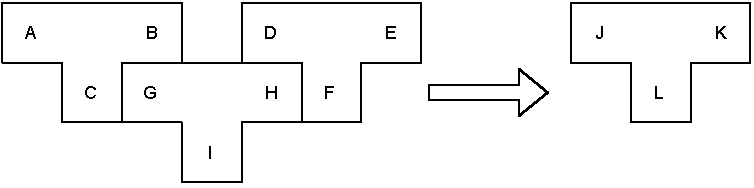
\includegraphics[width=.8\textwidth]{17.pdf}
\end{center}

  请给出一个该图所描述归约的实例。
  \item 在\ref{sec:1-6}节的图\ref{fig:1-3}中移植编译器的另一种方法是:对编译器生成的中间代码使用解释程序,并完全去掉后端。PascalP-system使用的就是这种方法,Pascal P-system包括了生成p-code的Pascal编译器、“一般的”栈式机器的汇编代码,以及模拟执行p-code的p-code解释程序。Pascal编译器和p-code解释程序均用p-code编写。
  \begin{enumerate}
    \item 假设有一个Pascal P-system,请描述在任一台机器上得到可运行的Pascal编译器的步骤。
    \item 描述在(a)中从你的系统得到一个可运行的本机代码编译器必需的步骤(也就是,为主机生成可执行代码的编译器,但不使用p-code解释程序)。
  \end{enumerate}
  \item 可以认为移植编译器的过程有两个不同的操作:重置目标(retargeting)(为新机器修改编译器以生成目标代码)和重置主机(rehosting)(修改编译程序以在新机器上运行)。请根据T型图讨论两个操作的不同之处。
\end{enumerate}

\section{笔记和参考}
\label{sec:1-10}

本章所讲到的大部分问题都将在以后各章中更加详细地再次提到,并且在以后的“笔记和参考”中也会给出恰当的参考。例如,第\ref{chap:2}章会谈到Lex,第\ref{chap:5}章中则是Yacc,第\ref{chap:6}章中是类型检查、符号表和属性分析,第\ref{chap:8}章中则为代码生成、三地址码和p-code,第\ref{chap:4}章和第\ref{chap:5}章会研究错误处理。

\citeauthoryear{aho2007compilers}是编译器的一个标准的综合参考,尤其是在理论和算法方面。\citeauthoryear{fischer1991crafting}中有许多有用的实行提示。在\citeauthoryear{fraser1995retargetable}和\citeauthoryear{holub1990compiler}中可找到对C编译器的完整描述。GNU编译器是一个源代码在Internet上广泛应用的流行的C/C++编译器,\citeauthoryear{stallman1994using}详细描述了它。

如果想要了解程序设计语言的概念以及程序设计语言和翻译程序之间交互的相关信息,可以参考\citeauthoryear{louden2011programming}或者\citeauthoryear{sethi1996programming}。

想要了解从数学的角度描述自动机理论,可以参考\citeauthoryear{hopcroft2001introduction}(和本书从实用的角度描述自动机理论有所不同)。从书中还可以找到更多的有关乔姆斯基层次结构的内容(第\ref{chap:3}章中也会提到)。

\citeauthoryear{backus1957fortran}和\citeauthoryear{backus1978history}中有对早期FORTRAN编译器的描述。在\citeauthoryear{randell1964algol}中有对早期的Algol 60编译器的描述。\citeauthoryear{barron1981pascal}描述了Pascal编译器,在这里还提到了Pascal P-system(\citeauthoryear{nori1981pascal})。

\citeauthoryear{kernighan1975ratfor}中有\ref{sec:1-2}节中提到的Ratfor预处理器,\citeauthoryear{bratman1961alternate}介绍了\ref{sec:1-6}节的T型图。

本书着重于对大多数语言的翻译中有用的标准翻译技术。要对在基于Algol命令语言的主要传统语言之外的语言进行有效的翻译可能还需要其他技术。特别地,用于诸如ML和Haskell的函数语言翻译已经发展了许多新技术,其中一些可能会成为将来重要的通用技术。\citeauthoryear{appel2007compiling}、\citeauthoryear{peyton1992implementing}和\citeauthoryear{peyton1987implementation}均提到了这些技术。\citeauthoryear{peyton1987implementation}还描述了Hindley-Milner类型检查(\ref{sec:1-1}节中已讲到过)。

\chapter{词法分析}
\label{chap:2}

\section{扫描处理}
\label{sec:2-1}

\section{正则表达式}
\label{sec:2-2}

\section{有限自动机}
\label{sec:2-3}

\section{从正则表达式到DFA}
\label{sec:2-4}

\section{TINY扫描器的实现}
\label{sec:2-5}

\section{利用Lex自动生成扫描器}
\label{sec:2-6}

\subsection{正则表达式的Lex约定}

\subsection{Lex输入文件的格式}

\subsection{使用Lex的TINY扫描器}

\chapter{上下文无关文法和语法分析}
\label{chap:3}

\section{语法分析的过程}
\label{sec:3-1}

\section{上下文无关文法}
\label{sec:3-2}

\section{语法分析树和抽象语法树}
\label{sec:3-3}

\section{二义性}
\label{sec:3-4}

\section{扩展表示法:EBNF和语法流程图}
\label{sec:3-5}

\section{上下文无关文法的形式化属性}
\label{sec:3-6}

\section{TINY语言的语法}
\label{sec:3-7}

\chapter{自顶向下语法分析}
\label{chap:4}

\section{使用递归下降语法分析算法进行自顶向下语法分析}
\label{sec:4-1}

\section{LL(1)语法分析}
\label{sec:4-2}

\section{First集合和Follow集合}
\label{sec:4-3}

\section{TINY语言的递归下降语法分析程序}
\label{sec:4-4}

\section{自顶向下语法分析程序中的错误校正}
\label{sec:4-5}

\chapter{自底向上语法分析}
\label{chap:5}

\section{自底向上语法分析概览}
\label{sec:5-1}

\section{LR(0)项的有限自动机与LR(0)语法分析}
\label{sec:5-2}

\section{SLR(1)语法分析}
\label{sec:5-3}

\section{一般的LR(1)和LALR(1)分析}
\label{sec:5-4}

\section{Yacc:一个LALR(1)的语法分析器生成器}
\label{sec:5-5}

\section{使用Yacc生成TINY语法分析器}
\label{sec:5-6}

\section{自底向上语法分析程序中的错误校正}
\label{sec:5-7}

\chapter{语义分析}
\label{chap:6}

\section{属性和属性语法}
\label{sec:6-1}

\section{属性计算算法}
\label{sec:6-2}

\section{符号表}
\label{sec:6-3}

\section{数据类型和类型检查}
\label{sec:6-4}

\section{TINY语言的语义分析}
\label{sec:6-5}

\chapter{运行时环境}
\label{chap:7}

\chapter{代码生成}
\label{chap:8}

\appendix

\chapter{一个编译器项目}
\label{append:A}

\section{C-Minus的词法约定}

\section{C-Minus的语法和语义}

\section{C-Minus的示例程序}

\section{C-Minus的Tiny Machine运行时环境}

\section{使用C-Minus和TM的编程项目}

\chapter{TINY编译器源码}
\label{append:B}

\begin{lstlisting}[caption={main.c},language=c]
/**************************/
/*   TINY编译器的主程序   */
/**************************/

#include "globals.h"

/* 将NO_PARSE设置为TRUE,编译器将只有扫描器功能 */
#define NO_PARSE FALSE
/* 将NO_ANALYZE设置为TRUE,编译器将只有语法分析器功能 */
#define NO_ANALYZE FALSE

/* 将NO_CODE置为TRUE,编译器将禁用代码生成功能 */
#define NO_CODE FALSE

#include "util.h"
#if NO_PARSE
#include "scan.h"
#else
#include "parse.h"
#if !NO_ANALYZE
#include "analyze.h"
#if !NO_CODE
#include "cgen.h"
#endif
#endif
#endif

/* 初始化一些全局变量 */
int lineno = 0;
FILE* source;
FILE* listing;
FILE* code;

/* 初始化一些追踪标志位 */
int EchoSource = FALSE;
int TraceScan = FALSE;
int TraceParse = FALSE;
int TraceAnalyze = FALSE;
int TraceCode = FALSE;

int Error = FALSE;

int main(int argc, char* argv[]) {
  TreeNode * syntaxTree;
  char pgm[120]; /* 源代码文件名 */
  if (argc != 2) {
    fprintf(stderr,"usage: %s <filename>\n",argv[0]);
    exit(1);
  }
  strcpy(pgm,argv[1]) ;
  if (strchr(pgm, '.') == NULL)
    strcat(pgm, ".tny");
  source = fopen(pgm, "r");
  if (source == NULL) {
    fprintf(stderr,"File %s not found\n",pgm);
    exit(1);
  }
  listing = stdout; /* send listing to screen */
  fprintf(listing, "\nTINY COMPILATION: %s\n", pgm);
#if NO_PARSE
  while (getToken() != ENDFILE);
#else
  syntaxTree = parse();
  if (TraceParse) {
    fprintf(listing, "\nSyntax tree:\n");
    printTree(syntaxTree);
  }
#if !NO_ANALYZE
  if (!Error) {
    if (TraceAnalyze) fprintf(listing, "\nBuilding Symbol Table...\n");
    buildSymtab(syntaxTree);
    if (TraceAnalyze) fprintf(listing, "\nChecking Types...\n");
    typeCheck(syntaxTree);
    if (TraceAnalyze) fprintf(listing, "\nType Checking Finished\n");
  }
#if !NO_CODE
  if (!Error) {
    char* codefile;
    int fnlen = strcspn(pgm, ".");
    codefile = (char *)calloc(fnlen+4, sizeof(char));
    strncpy(codefile, pgm, fnlen);
    strcat(codefile, ".tm");
    code = fopen(codefile, "w");
    if (code == NULL) {
      printf("Unable to open %s\n", codefile);
      exit(1);
    }
    codeGen(syntaxTree, codefile);
    fclose(code);
  }
#endif
#endif
#endif
  fclose(source);
  return 0;
}
\end{lstlisting}

\begin{lstlisting}[caption={globals.h},language=c]
#ifndef _GLOBALS_H_
#define _GLOBALS_H_

#include <stdio.h>
#include <stdlib.h>
#include <ctype.h>
#include <string.h>

#ifndef FALSE
#define FALSE 0
#endif

#ifndef TRUE
#define TRUE 1
#endif

/* MAXRESERVED = 关键字数量 */
#define MAXRESERVED 8

typedef enum {
  ENDFILE, // 文件结束符
  ERROR,   // 错误记号
  IF,      // if
  THEN,    // then
  ELSE,    // else
  END,     // end
  REPEAT,  // repeat
  UNTIL,   // until
  READ,    // read
  WRITE,   // write
  ID,      // 标识符
  NUM,     // 数值
  ASSIGN,  // 赋值运算符`:=`
  EQ,      // ==
  LT,      // <
  PLUS,    // +
  MINUS,   // -
  TIMES,   // *
  OVER,    // `/`
  LPAREN,  // (
  RPAREN,  // )
  SEMI     // ;
} TokenType;

extern FILE* source; /* 源代码文件 */
extern FILE* listing; /* listing output text file */
extern FILE* code; /* code text file for TM simulator */

extern int lineno; /* 源代码行号 */

/**************************************************/
/***********   语法树(语法分析使用)  ************/
/**************************************************/

typedef enum {
  StmtK,
  ExpK
} NodeKind;

typedef enum {
  IfK,
  RepeatK,
  AssignK,
  ReadK,
  WriteK
} StmtKind;

typedef enum {
  OpK,
  ConstK,
  IdK
} ExpKind;

/* ExpType is used for type checking */
typedef enum {
  Void,
  Integer,
  Boolean
} ExpType;

#define MAXCHILDREN 3

typedef struct treeNode {
  struct treeNode* child[MAXCHILDREN];
  struct treeNode* sibling;
  int lineno;
  NodeKind nodekind;
  union {
    StmtKind stmt;
    ExpKind exp;
  } kind;
  union {
    TokenType op;
    int val;
    char* name;
  } attr;
  ExpType type; /* for type checking of exps */
} TreeNode;

/**************************************************/
/***********   Flags for tracing       ************/
/**************************************************/

/* EchoSource = TRUE causes the source program to
 * be echoed to the listing file with line numbers
 * during parsing
 */
extern int EchoSource;

/* TraceScan = TRUE causes token information to be
 * printed to the listing file as each token is
 * recognized by the scanner
 */
extern int TraceScan;

/* TraceParse = TRUE causes the syntax tree to be
 * printed to the listing file in linearized form
 * (using indents for children)
 */
extern int TraceParse;

/* TraceAnalyze = TRUE causes symbol table inserts
 * and lookups to be reported to the listing file
 */
extern int TraceAnalyze;

/* TraceCode = TRUE causes comments to be written
 * to the TM code file as code is generated
 */
extern int TraceCode;

/* Error = TRUE prevents further passes if an error occurs */
extern int Error; 
#endif
\end{lstlisting}

\begin{lstlisting}[caption={util.h},language=c]
#ifndef _UTIL_H_
#define _UTIL_H_

/* Procedure printToken prints a token 
 * and its lexeme to the listing file
 */
void printToken(TokenType, const char*);

/* Function newStmtNode creates a new statement
 * node for syntax tree construction
 */
TreeNode* newStmtNode(StmtKind);

/* Function newExpNode creates a new expression 
 * node for syntax tree construction
 */
TreeNode* newExpNode(ExpKind);

/* Function copyString allocates and makes a new
 * copy of an existing string
 */
char* copyString(char*);

/* procedure printTree prints a syntax tree to the 
 * listing file using indentation to indicate subtrees
 */
void printTree(TreeNode*);

#endif
\end{lstlisting}

\begin{lstlisting}[caption={util.c},language=c]
#include "globals.h"
#include "util.h"

/* Procedure printToken prints a token 
 * and its lexeme to the listing file
 */
void printToken(TokenType token, const char* tokenString) {
  switch (token) {
    case IF:
    case THEN:
    case ELSE:
    case END:
    case REPEAT:
    case UNTIL:
    case READ:
    case WRITE:
      fprintf(listing, "reserved word: %s\n", tokenString);
      break;
    case ASSIGN: fprintf(listing, ":=\n"); break;
    case LT: fprintf(listing, "<\n"); break;
    case EQ: fprintf(listing, "=\n"); break;
    case LPAREN: fprintf(listing, "(\n"); break;
    case RPAREN: fprintf(listing, ")\n"); break;
    case SEMI: fprintf(listing, ";\n"); break;
    case PLUS: fprintf(listing, "+\n"); break;
    case MINUS: fprintf(listing, "-\n"); break;
    case TIMES: fprintf(listing, "*\n"); break;
    case OVER: fprintf(listing, "/\n"); break;
    case ENDFILE: fprintf(listing, "EOF\n"); break;
    case NUM:
      fprintf(listing, "NUM, val= %s\n", tokenString);
      break;
    case ID:
      fprintf(listing, "ID, name= %s\n", tokenString);
      break;
    case ERROR:
      fprintf(listing, "ERROR: %s\n", tokenString);
      break;
    default: /* should never happen */
      fprintf(listing, "Unknown token: %d\n", token);
  }
}

/* Function newStmtNode creates a new statement
 * node for syntax tree construction
 */
TreeNode* newStmtNode(StmtKind kind) {
  TreeNode* t = (TreeNode*)malloc(sizeof(TreeNode));
  int i;
  if (t == NULL)
    fprintf(listing, "Out of memory error at line %d\n", lineno);
  else {
    for (i = 0; i < MAXCHILDREN; i++) t->child[i] = NULL;
    t->sibling = NULL;
    t->nodekind = StmtK;
    t->kind.stmt = kind;
    t->lineno = lineno;
  }
  return t;
}

/* Function newExpNode creates a new expression 
 * node for syntax tree construction
 */
TreeNode* newExpNode(ExpKind kind) {
  TreeNode* t = (TreeNode*)malloc(sizeof(TreeNode));
  int i;
  if (t == NULL)
    fprintf(listing, "Out of memory error at line %d\n", lineno);
  else {
    for (i = 0; i < MAXCHILDREN; i++) t->child[i] = NULL;
    t->sibling = NULL;
    t->nodekind = ExpK;
    t->kind.exp = kind;
    t->lineno = lineno;
    t->type = Void;
  }
  return t;
}

/* Function copyString allocates and makes a new
 * copy of an existing string
 */
char* copyString(char* s) {
  int n;
  char* t;
  if (s == NULL) return NULL;
  n = strlen(s) + 1;
  t = malloc(n);
  if (t == NULL)
    fprintf(listing, "Out of memory error at line %d\n", lineno);
  else strcpy(t, s);
  return t;
}

/* Variable indentno is used by printTree to
 * store current number of spaces to indent
 */
static indentno = 0;

/* macros to increase/decrease indentation */
#define INDENT indentno += 2
#define UNINDENT indentno -= 2

/* printSpaces indents by printing spaces */
static void printSpaces(void) {
  int i;
  for (i = 0; i < indentno; i++)
    fprintf(listing, " ");
}

/* procedure printTree prints a syntax tree to the 
 * listing file using indentation to indicate subtrees
 */
void printTree(TreeNode* tree) {
  int i;
  INDENT;
  while (tree != NULL) {
    printSpaces();
    if (tree->nodekind == StmtK) {
      switch (tree->kind.stmt) {
        case IfK:
          fprintf(listing, "If\n");
          break;
        case RepeatK:
          fprintf(listing, "Repeat\n");
          break;
        case AssignK:
          fprintf(listing, "Assign to: %s\n", tree->attr.name);
          break;
        case ReadK:
          fprintf(listing, "Read: %s\n", tree->attr.name);
          break;
        case WriteK:
          fprintf(listing, "Write\n");
          break;
        default:
          fprintf(listing, "Unknown ExpNode kind\n");
          break;
      }
    } else if (tree->nodekind == ExpK) {
      switch (tree->kind.exp) {
        case OpK:
          fprintf(listing, "Op: ");
          printToken(tree->attr.op, "\0");
          break;
        case ConstK:
          fprintf(listing, "Const: %d\n", tree->attr.val);
          break;
        case IdK:
          fprintf(listing, "Id: %s\n", tree->attr.name);
          break;
        default:
          fprintf(listing, "Unknown ExpNode kind\n");
          break;
      }
    } else {
      fprintf(listing, "Unknown node kind\n");
    }
    for (i = 0; i < MAXCHILDREN; i++)
      printTree(tree->child[i]);
    tree = tree->sibling;
  }
  UNINDENT;
}
\end{lstlisting}

\begin{lstlisting}[caption={scan.h},language=c]
#ifndef _SCAN_H_
#define _SCAN_H_

/* MAXTOKENLEN is the maximum size of a token */
#define MAXTOKENLEN 40

/* tokenString array stores the lexeme of each token */
extern char tokenString[MAXTOKENLEN+1];

/* function getToken returns the 
 * next token in source file
 */
TokenType getToken(void);

#endif
\end{lstlisting}

\begin{lstlisting}[caption={scan.c},language=c]
#include "globals.h"
#include "util.h"
#include "scan.h"

/* states in scanner DFA */
typedef enum {
  START,
  INASSIGN,
  INCOMMENT,
  INNUM,
  INID,
  DONE
} StateType;

/* lexeme of identifier or reserved word */
char tokenString[MAXTOKENLEN+1];

/* BUFLEN = length of the input buffer for
   source code lines */
#define BUFLEN 256

static char lineBuf[BUFLEN]; /* holds the current line */
static int linepos = 0; /* current position in LineBuf */
static int bufsize = 0; /* current size of buffer string */
static int EOF_flag = FALSE; /* corrects ungetNextChar behavior on EOF */

/* getNextChar fetches the next non-blank character
   from lineBuf, reading in a new line if lineBuf is
   exhausted */
static int getNextChar(void) {
  if (!(linepos < bufsize)) {
    lineno++;
    if (fgets(lineBuf,BUFLEN-1,source)) {
      if (EchoSource) fprintf(listing, "%4d: %s", lineno, lineBuf);
      bufsize = strlen(lineBuf);
      linepos = 0;
      return lineBuf[linepos++];
    } else {
      EOF_flag = TRUE;
      return EOF;
    }
  }
  else return lineBuf[linepos++];
}

/* ungetNextChar backtracks one character
   in lineBuf */
static void ungetNextChar(void) {
  if (!EOF_flag) linepos--;
}

/* lookup table of reserved words */
static struct
    { char* str;
      TokenType tok;
    } reservedWords[MAXRESERVED]
   = {{"if",IF},{"then",THEN},{"else",ELSE},{"end",END},
      {"repeat",REPEAT},{"until",UNTIL},{"read",READ},
      {"write",WRITE}};

/* lookup an identifier to see if it is a reserved word */
/* uses linear search */
static TokenType reservedLookup (char * s) {
  int i;
  for (i = 0; i < MAXRESERVED; i++)
    if (!strcmp(s, reservedWords[i].str))
      return reservedWords[i].tok;
  return ID;
}

/****************************************/
/* the primary function of the scanner  */
/****************************************/
/* function getToken returns the 
 * next token in source file
 */
TokenType getToken(void) {
  /* index for storing into tokenString */
   int tokenStringIndex = 0;
   /* holds current token to be returned */
   TokenType currentToken;
   /* current state - always begins at START */
   StateType state = START;
   /* flag to indicate save to tokenString */
   int save;
   while (state != DONE)
   { int c = getNextChar();
     save = TRUE;
     switch (state)
     { case START:
         if (isdigit(c))
           state = INNUM;
         else if (isalpha(c))
           state = INID;
         else if (c == ':')
           state = INASSIGN;
         else if ((c == ' ') || (c == '\t') || (c == '\n'))
           save = FALSE;
         else if (c == '{')
         { save = FALSE;
           state = INCOMMENT;
         }
         else
         { state = DONE;
           switch (c)
           { case EOF:
               save = FALSE;
               currentToken = ENDFILE;
               break;
             case '=':
               currentToken = EQ;
               break;
             case '<':
               currentToken = LT;
               break;
             case '+':
               currentToken = PLUS;
               break;
             case '-':
               currentToken = MINUS;
               break;
             case '*':
               currentToken = TIMES;
               break;
             case '/':
               currentToken = OVER;
               break;
             case '(':
               currentToken = LPAREN;
               break;
             case ')':
               currentToken = RPAREN;
               break;
             case ';':
               currentToken = SEMI;
               break;
             default:
               currentToken = ERROR;
               break;
           }
         }
         break;
       case INCOMMENT:
         save = FALSE;
         if (c == EOF)
         { state = DONE;
           currentToken = ENDFILE;
         }
         else if (c == '}') state = START;
         break;
       case INASSIGN:
         state = DONE;
         if (c == '=')
           currentToken = ASSIGN;
         else
         { /* backup in the input */
           ungetNextChar();
           save = FALSE;
           currentToken = ERROR;
         }
         break;
       case INNUM:
         if (!isdigit(c))
         { /* backup in the input */
           ungetNextChar();
           save = FALSE;
           state = DONE;
           currentToken = NUM;
         }
         break;
       case INID:
         if (!isalpha(c))
         { /* backup in the input */
           ungetNextChar();
           save = FALSE;
           state = DONE;
           currentToken = ID;
         }
         break;
       case DONE:
       default: /* should never happen */
         fprintf(listing,"Scanner Bug: state= %d\n",state);
         state = DONE;
         currentToken = ERROR;
         break;
     }
     if ((save) && (tokenStringIndex <= MAXTOKENLEN))
       tokenString[tokenStringIndex++] = (char) c;
     if (state == DONE)
     { tokenString[tokenStringIndex] = '\0';
       if (currentToken == ID)
         currentToken = reservedLookup(tokenString);
     }
   }
   if (TraceScan) {
     fprintf(listing,"\t%d: ",lineno);
     printToken(currentToken,tokenString);
   }
   return currentToken;
} /* end getToken */
\end{lstlisting}

\begin{lstlisting}[caption={parse.h},language=c]
#ifndef _PARSE_H_
#define _PARSE_H_

/* Function parse returns the newly 
 * constructed syntax tree
 */
TreeNode* parse(void);

#endif
\end{lstlisting}

\begin{lstlisting}[caption={parse.c},language=c]
#include "globals.h"
#include "util.h"
#include "scan.h"
#include "parse.h"

static TokenType token; /* holds current token */

/* function prototypes for recursive calls */
static TreeNode * stmt_sequence(void);
static TreeNode * statement(void);
static TreeNode * if_stmt(void);
static TreeNode * repeat_stmt(void);
static TreeNode * assign_stmt(void);
static TreeNode * read_stmt(void);
static TreeNode * write_stmt(void);
static TreeNode * exp(void);
static TreeNode * simple_exp(void);
static TreeNode * term(void);
static TreeNode * factor(void);

static void syntaxError(char* message) {
  fprintf(listing, "\n>>> ");
  fprintf(listing, "Syntax error at line %d: %s", lineno, message);
  Error = TRUE;
}

static void match(TokenType expected) {
  if (token == expected) token = getToken();
  else {
    syntaxError("unexpected token -> ");
    printToken(token, tokenString);
    fprintf(listing, "      ");
  }
}

TreeNode* stmt_sequence(void) {
  TreeNode* t = statement();
  TreeNode* p = t;
  while ((token!=ENDFILE) && (token!=END) &&
         (token!=ELSE) && (token!=UNTIL)) {
    TreeNode* q;
    match(SEMI);
    q = statement();
    if (q != NULL) {
      if (t == NULL) t = p = q;
      else {
        /* now p cannot be NULL either */
        p->sibling = q;
        p = q;
      }
    }
  }
  return t;
}

TreeNode* statement(void) {
  TreeNode* t = NULL;
  switch (token) {
    case IF: t = if_stmt(); break;
    case REPEAT: t = repeat_stmt(); break;
    case ID: t = assign_stmt(); break;
    case READ: t = read_stmt(); break;
    case WRITE: t = write_stmt(); break;
    default:
      syntaxError("unexpected token -> ");
      printToken(token,tokenString);
      token = getToken();
      break;
  } /* end case */
  return t;
}

TreeNode* if_stmt(void) {
  TreeNode* t = newStmtNode(IfK);
  match(IF);
  if (t != NULL) t->child[0] = exp();
  match(THEN);
  if (t != NULL) t->child[1] = stmt_sequence();
  if (token==ELSE) {
    match(ELSE);
    if (t != NULL) t->child[2] = stmt_sequence();
  }
  match(END);
  return t;
}

TreeNode* repeat_stmt(void) {
  TreeNode* t = newStmtNode(RepeatK);
  match(REPEAT);
  if (t != NULL) t->child[0] = stmt_sequence();
  match(UNTIL);
  if (t != NULL) t->child[1] = exp();
  return t;
}

TreeNode * assign_stmt(void)
{ TreeNode * t = newStmtNode(AssignK);
  if ((t!=NULL) && (token==ID))
    t->attr.name = copyString(tokenString);
  match(ID);
  match(ASSIGN);
  if (t!=NULL) t->child[0] = exp();
  return t;
}

TreeNode * read_stmt(void)
{ TreeNode * t = newStmtNode(ReadK);
  match(READ);
  if ((t!=NULL) && (token==ID))
    t->attr.name = copyString(tokenString);
  match(ID);
  return t;
}

TreeNode * write_stmt(void)
{ TreeNode * t = newStmtNode(WriteK);
  match(WRITE);
  if (t!=NULL) t->child[0] = exp();
  return t;
}

TreeNode * exp(void)
{ TreeNode * t = simple_exp();
  if ((token==LT)||(token==EQ)) {
    TreeNode * p = newExpNode(OpK);
    if (p!=NULL) {
      p->child[0] = t;
      p->attr.op = token;
      t = p;
    }
    match(token);
    if (t!=NULL)
      t->child[1] = simple_exp();
  }
  return t;
}

TreeNode * simple_exp(void)
{ TreeNode * t = term();
  while ((token==PLUS)||(token==MINUS))
  { TreeNode * p = newExpNode(OpK);
    if (p!=NULL) {
      p->child[0] = t;
      p->attr.op = token;
      t = p;
      match(token);
      t->child[1] = term();
    }
  }
  return t;
}

TreeNode* term(void) {
  TreeNode* t = factor();
  while ((token == TIMES) || (token == OVER)) {
    TreeNode* p = newExpNode(OpK);
    if (p != NULL) {
      p->child[0] = t;
      p->attr.op = token;
      t = p;
      match(token);
      p->child[1] = factor();
    }
  }
  return t;
}

TreeNode* factor(void) {
  TreeNode* t = NULL;
  switch (token) {
    case NUM:
      t = newExpNode(ConstK);
      if ((t != NULL) && (token == NUM))
        t->attr.val = atoi(tokenString);
      match(NUM);
      break;
    case ID:
      t = newExpNode(IdK);
      if ((t != NULL) && (token == ID))
        t->attr.name = copyString(tokenString);
      match(ID);
      break;
    case LPAREN:
      match(LPAREN);
      t = exp();
      match(RPAREN);
      break;
    default:
      syntaxError("unexpected token -> ");
      printToken(token, tokenString);
      token = getToken();
      break;
    }
  return t;
}

/****************************************/
/* the primary function of the parser   */
/****************************************/
/* Function parse returns the newly 
 * constructed syntax tree
 */
TreeNode* parse(void) {
  TreeNode* t;
  token = getToken();
  t = stmt_sequence();
  if (token != ENDFILE)
    syntaxError("Code ends before file\n");
  return t;
}
\end{lstlisting}

\begin{lstlisting}[caption={symtab.h},language=c]
#ifndef _SYMTAB_H_
#define _SYMTAB_H_

/* Procedure st_insert inserts line numbers and
 * memory locations into the symbol table
 * loc = memory location is inserted only the
 * first time, otherwise ignored
 */
void st_insert(char* name, int lineno, int loc);

/* Function st_lookup returns the memory 
 * location of a variable or -1 if not found
 */
int st_lookup (char* name);

/* Procedure printSymTab prints a formatted 
 * listing of the symbol table contents 
 * to the listing file
 */
void printSymTab(FILE* listing);

#endif
\end{lstlisting}

\begin{lstlisting}[caption={symtab.c},language=c]
#include <stdio.h>
#include <stdlib.h>
#include <string.h>
#include "symtab.h"

/* SIZE is the size of the hash table */
#define SIZE 211

/* SHIFT is the power of two used as multiplier
   in hash function  */
#define SHIFT 4

/* the hash function */
static int hash (char* key) {
  int temp = 0;
  int i = 0;
  while (key[i] != '\0') {
    temp = ((temp << SHIFT) + key[i]) % SIZE;
    ++i;
  }
  return temp;
}

/* the list of line numbers of the source 
 * code in which a variable is referenced
 */
typedef struct LineListRec {
  int lineno;
  struct LineListRec * next;
} *LineList;

/* The record in the bucket lists for
 * each variable, including name, 
 * assigned memory location, and
 * the list of line numbers in which
 * it appears in the source code
 */
typedef struct BucketListRec {
  char * name;
  LineList lines;
  int memloc ; /* memory location for variable */
  struct BucketListRec * next;
} *BucketList;

/* the hash table */
static BucketList hashTable[SIZE];

/* Procedure st_insert inserts line numbers and
 * memory locations into the symbol table
 * loc = memory location is inserted only the
 * first time, otherwise ignored
 */
void st_insert(char* name, int lineno, int loc) {
  int h = hash(name);
  BucketList l =  hashTable[h];
  while ((l != NULL) && (strcmp(name,l->name) != 0))
    l = l->next;
  if (l == NULL) {
    /* variable not yet in table */
    l = (BucketList) malloc(sizeof(struct BucketListRec));
    l->name = name;
    l->lines = (LineList) malloc(sizeof(struct LineListRec));
    l->lines->lineno = lineno;
    l->memloc = loc;
    l->lines->next = NULL;
    l->next = hashTable[h];
    hashTable[h] = l;
  } else {
    /* found in table, so just add line number */
    LineList t = l->lines;
    while (t->next != NULL) t = t->next;
    t->next = (LineList) malloc(sizeof(struct LineListRec));
    t->next->lineno = lineno;
    t->next->next = NULL;
  }
} /* st_insert */

/* Function st_lookup returns the memory 
 * location of a variable or -1 if not found
 */
int st_lookup(char* name) {
  int h = hash(name);
  BucketList l =  hashTable[h];
  while ((l != NULL) && (strcmp(name,l->name) != 0))
    l = l->next;
  if (l == NULL) return -1;
  else return l->memloc;
}

/* Procedure printSymTab prints a formatted 
 * listing of the symbol table contents 
 * to the listing file
 */
void printSymTab(FILE* listing) {
  int i;
  fprintf(listing,"Variable Name  Location   Line Numbers\n");
  fprintf(listing,"-------------  --------   ------------\n");
  for (i = 0; i < SIZE; ++i) {
    if (hashTable[i] != NULL) {
      BucketList l = hashTable[i];
      while (l != NULL) {
        LineList t = l->lines;
        fprintf(listing, "%-14s ", l->name);
        fprintf(listing, "%-8d  ", l->memloc);
        while (t != NULL) {
          fprintf(listing,"%4d ",t->lineno);
          t = t->next;
        }
        fprintf(listing,"\n");
        l = l->next;
      }
    }
  }
} /* printSymTab */
\end{lstlisting}

\begin{lstlisting}[caption={analyze.h},language=c]
#ifndef _ANALYZE_H_
#define _ANALYZE_H_

/* Function buildSymtab constructs the symbol 
 * table by preorder traversal of the syntax tree
 */
void buildSymtab(TreeNode*);

/* Procedure typeCheck performs type checking 
 * by a postorder syntax tree traversal
 */
void typeCheck(TreeNode*);

#endif
\end{lstlisting}

\begin{lstlisting}[caption={analyze.c},language=c]
#include "globals.h"
#include "symtab.h"
#include "analyze.h"

/* counter for variable memory locations */
static int location = 0;

/* Procedure traverse is a generic recursive 
 * syntax tree traversal routine:
 * it applies preProc in preorder and postProc 
 * in postorder to tree pointed to by t
 */
static void traverse(TreeNode* t,
               void(*preProc) (TreeNode*),
               void(*postProc) (TreeNode*)) {
  if (t != NULL) {
    preProc(t);
    {
      int i;
      for (i=0; i < MAXCHILDREN; i++)
        traverse(t->child[i],preProc,postProc);
    }
    postProc(t);
    traverse(t->sibling,preProc,postProc);
  }
}

/* nullProc is a do-nothing procedure to 
 * generate preorder-only or postorder-only
 * traversals from traverse
 */
static void nullProc(TreeNode* t) {
  if (t == NULL) return;
  else return;
}

/* Procedure insertNode inserts 
 * identifiers stored in t into 
 * the symbol table 
 */
static void insertNode(TreeNode* t) {
  switch (t->nodekind) {
    case StmtK:
      switch (t->kind.stmt) {
        case AssignK:
        case ReadK:
          if (st_lookup(t->attr.name) == -1)
          /* not yet in table, so treat as new definition */
            st_insert(t->attr.name,t->lineno,location++);
          else
          /* already in table, so ignore location, 
             add line number of use only */ 
            st_insert(t->attr.name,t->lineno,0);
          break;
        default:
          break;
      }
      break;
    case ExpK:
      switch (t->kind.exp) {
        case IdK:
          if (st_lookup(t->attr.name) == -1)
          /* not yet in table, so treat as new definition */
            st_insert(t->attr.name,t->lineno,location++);
          else
          /* already in table, so ignore location, 
             add line number of use only */ 
            st_insert(t->attr.name,t->lineno,0);
          break;
        default:
          break;
      }
      break;
    default:
      break;
  }
}

/* Function buildSymtab constructs the symbol 
 * table by preorder traversal of the syntax tree
 */
void buildSymtab(TreeNode * syntaxTree)
{ traverse(syntaxTree,insertNode,nullProc);
  if (TraceAnalyze)
  { fprintf(listing,"\nSymbol table:\n\n");
    printSymTab(listing);
  }
}

static void typeError(TreeNode* t, char* message) {
  fprintf(listing,"Type error at line %d: %s\n",t->lineno,message);
  Error = TRUE;
}

/* Procedure checkNode performs
 * type checking at a single tree node
 */
static void checkNode(TreeNode* t) {
  switch (t->nodekind) {
    case ExpK:
      switch (t->kind.exp) {
        case OpK:
          if ((t->child[0]->type != Integer) ||
              (t->child[1]->type != Integer))
            typeError(t,"Op applied to non-integer");
          if ((t->attr.op == EQ) || (t->attr.op == LT))
            t->type = Boolean;
          else
            t->type = Integer;
          break;
        case ConstK:
        case IdK:
          t->type = Integer;
          break;
        default:
          break;
      }
      break;
    case StmtK:
      switch (t->kind.stmt) {
        case IfK:
          if (t->child[0]->type == Integer)
            typeError(t->child[0],"if test is not Boolean");
          break;
        case AssignK:
          if (t->child[0]->type != Integer)
            typeError(t->child[0],"assignment of non-integer value");
          break;
        case WriteK:
          if (t->child[0]->type != Integer)
            typeError(t->child[0],"write of non-integer value");
          break;
        case RepeatK:
          if (t->child[1]->type == Integer)
            typeError(t->child[1],"repeat test is not Boolean");
          break;
        default:
          break;
      }
      break;
    default:
      break;
  }
}

/* Procedure typeCheck performs type checking 
 * by a postorder syntax tree traversal
 */
void typeCheck(TreeNode * syntaxTree) {
  traverse(syntaxTree, nullProc, checkNode);
}
\end{lstlisting}

\begin{lstlisting}[caption={code.h},language=c]
#ifndef _CODE_H_
#define _CODE_H_

/* pc = program counter  */
#define pc 7

/* mp = "memory pointer" points
 * to top of memory (for temp storage)
 */
#define mp 6

/* gp = "global pointer" points
 * to bottom of memory for (global)
 * variable storage
 */
#define gp 5

/* accumulator */
#define ac 0

/* 2nd accumulator */
#define ac1 1

/* code emitting utilities */

/* Procedure emitComment prints a comment line 
 * with comment c in the code file
 */
void emitComment(char* c);

/* Procedure emitRO emits a register-only
 * TM instruction
 * op = the opcode
 * r = target register
 * s = 1st source register
 * t = 2nd source register
 * c = a comment to be printed if TraceCode is TRUE
 */
void emitRO(char *op, int r, int s, int t, char *c);

/* Procedure emitRM emits a register-to-memory
 * TM instruction
 * op = the opcode
 * r = target register
 * d = the offset
 * s = the base register
 * c = a comment to be printed if TraceCode is TRUE
 */
void emitRM(char* op, int r, int d, int s, char* c);

/* Function emitSkip skips "howMany" code
 * locations for later backpatch. It also
 * returns the current code position
 */
int emitSkip(int howMany);

/* Procedure emitBackup backs up to 
 * loc = a previously skipped location
 */
void emitBackup(int loc);

/* Procedure emitRestore restores the current 
 * code position to the highest previously
 * unemitted position
 */
void emitRestore(void);

/* Procedure emitRM_Abs converts an absolute reference 
 * to a pc-relative reference when emitting a
 * register-to-memory TM instruction
 * op = the opcode
 * r = target register
 * a = the absolute location in memory
 * c = a comment to be printed if TraceCode is TRUE
 */
void emitRM_Abs(char* op, int r, int a, char* c);

#endif
\end{lstlisting}

\begin{lstlisting}[caption={code.c},language=c]
#include "globals.h"
#include "code.h"

/* TM location number for current instruction emission */
static int emitLoc = 0;

/* Highest TM location emitted so far
   For use in conjunction with emitSkip,
   emitBackup, and emitRestore */
static int highEmitLoc = 0;

/* Procedure emitComment prints a comment line 
 * with comment c in the code file
 */
void emitComment(char* c ) {
  if (TraceCode) fprintf(code,"* %s\n",c);
}

/* Procedure emitRO emits a register-only
 * TM instruction
 * op = the opcode
 * r = target register
 * s = 1st source register
 * t = 2nd source register
 * c = a comment to be printed if TraceCode is TRUE
 */
void emitRO(char* op, int r, int s, int t, char* c) {
  fprintf(code,"%3d:  %5s  %d,%d,%d ",emitLoc++,op,r,s,t);
  if (TraceCode) fprintf(code,"\t%s",c) ;
  fprintf(code,"\n") ;
  if (highEmitLoc < emitLoc) highEmitLoc = emitLoc ;
} /* emitRO */

/* Procedure emitRM emits a register-to-memory
 * TM instruction
 * op = the opcode
 * r = target register
 * d = the offset
 * s = the base register
 * c = a comment to be printed if TraceCode is TRUE
 */
void emitRM(char* op, int r, int d, int s, char* c) {
  fprintf(code,"%3d:  %5s  %d,%d(%d) ",emitLoc++,op,r,d,s);
  if (TraceCode) fprintf(code,"\t%s",c) ;
  fprintf(code,"\n") ;
  if (highEmitLoc < emitLoc)  highEmitLoc = emitLoc ;
} /* emitRM */

/* Function emitSkip skips "howMany" code
 * locations for later backpatch. It also
 * returns the current code position
 */
int emitSkip(int howMany) { 
  int i = emitLoc;
  emitLoc += howMany;
  if (highEmitLoc < emitLoc)  highEmitLoc = emitLoc;
  return i;
} /* emitSkip */

/* Procedure emitBackup backs up to 
 * loc = a previously skipped location
 */
void emitBackup(int loc) {
  if (loc > highEmitLoc) emitComment("BUG in emitBackup");
  emitLoc = loc;
} /* emitBackup */

/* Procedure emitRestore restores the current 
 * code position to the highest previously
 * unemitted position
 */
void emitRestore(void) {
  emitLoc = highEmitLoc;
}

/* Procedure emitRM_Abs converts an absolute reference 
 * to a pc-relative reference when emitting a
 * register-to-memory TM instruction
 * op = the opcode
 * r = target register
 * a = the absolute location in memory
 * c = a comment to be printed if TraceCode is TRUE
 */
void emitRM_Abs(char* op, int r, int a, char* c) {
  fprintf(code,"%3d:  %5s  %d,%d(%d) ",
               emitLoc,op,r,a-(emitLoc+1),pc);
  ++emitLoc;
  if (TraceCode) fprintf(code,"\t%s",c) ;
  fprintf(code,"\n") ;
  if (highEmitLoc < emitLoc) highEmitLoc = emitLoc;
} /* emitRM_Abs */
\end{lstlisting}

\begin{lstlisting}[caption={cgen.h},language=c]
#ifndef _CGEN_H_
#define _CGEN_H_

/* Procedure codeGen generates code to a code
 * file by traversal of the syntax tree. The
 * second parameter (codefile) is the file name
 * of the code file, and is used to print the
 * file name as a comment in the code file
 */
void codeGen(TreeNode* syntaxTree, char* codefile);

#endif
\end{lstlisting}

\begin{lstlisting}[caption={cgen.c},language=c]
#include "globals.h"
#include "symtab.h"
#include "code.h"
#include "cgen.h"

/* tmpOffset is the memory offset for temps
   It is decremented each time a temp is
   stored, and incremeted when loaded again
*/
static int tmpOffset = 0;

/* prototype for internal recursive code generator */
static void cGen(TreeNode* tree);

/* Procedure genStmt generates code at a statement node */
static void genStmt(TreeNode* tree) {
  TreeNode *p1, *p2, *p3;
  int savedLoc1, savedLoc2, currentLoc;
  int loc;
  switch (tree->kind.stmt) {
      case IfK:
         if (TraceCode) emitComment("-> if");
         p1 = tree->child[0];
         p2 = tree->child[1];
         p3 = tree->child[2];
         /* generate code for test expression */
         cGen(p1);
         savedLoc1 = emitSkip(1);
         emitComment("if: jump to else belongs here");
         /* recurse on then part */
         cGen(p2);
         savedLoc2 = emitSkip(1);
         emitComment("if: jump to end belongs here");
         currentLoc = emitSkip(0);
         emitBackup(savedLoc1);
         emitRM_Abs("JEQ", ac, currentLoc, "if: jmp to else");
         emitRestore();
         /* recurse on else part */
         cGen(p3);
         currentLoc = emitSkip(0);
         emitBackup(savedLoc2);
         emitRM_Abs("LDA", pc, currentLoc, "jmp to end");
         emitRestore();
         if (TraceCode) emitComment("<- if");
         break; /* if_k */
      case RepeatK:
         if (TraceCode) emitComment("-> repeat");
         p1 = tree->child[0];
         p2 = tree->child[1];
         savedLoc1 = emitSkip(0);
         emitComment("repeat: jump after body comes back here");
         /* generate code for body */
         cGen(p1);
         /* generate code for test */
         cGen(p2);
         emitRM_Abs("JEQ", ac, savedLoc1, "repeat: jmp back to body");
         if (TraceCode)  emitComment("<- repeat");
         break; /* repeat */
      case AssignK:
         if (TraceCode) emitComment("-> assign");
         /* generate code for rhs */
         cGen(tree->child[0]);
         /* now store value */
         loc = st_lookup(tree->attr.name);
         emitRM("ST", ac, loc, gp, "assign: store value");
         if (TraceCode) emitComment("<- assign");
         break; /* assign_k */
      case ReadK:
         emitRO("IN", ac, 0, 0, "read integer value");
         loc = st_lookup(tree->attr.name);
         emitRM("ST", ac, loc, gp, "read: store value");
         break;
      case WriteK:
         /* generate code for expression to write */
         cGen(tree->child[0]);
         /* now output it */
         emitRO("OUT", ac, 0, 0, "write ac");
         break;
      default:
         break;
    }
} /* genStmt */

/* Procedure genExp generates code at an expression node */
static void genExp(TreeNode* tree) {
  int loc;
  TreeNode *p1, *p2;
  switch (tree->kind.exp) {
    case ConstK:
      if (TraceCode) emitComment("-> Const");
      /* gen code to load integer constant using LDC */
      emitRM("LDC",ac,tree->attr.val,0,"load const");
      if (TraceCode)  emitComment("<- Const");
      break; /* ConstK */
    
    case IdK:
      if (TraceCode) emitComment("-> Id");
      loc = st_lookup(tree->attr.name);
      emitRM("LD",ac,loc,gp,"load id value");
      if (TraceCode)  emitComment("<- Id");
      break; /* IdK */

    case OpK :
         if (TraceCode) emitComment("-> Op");
         p1 = tree->child[0];
         p2 = tree->child[1];
         /* gen code for ac = left arg */
         cGen(p1);
         /* gen code to push left operand */
         emitRM("ST",ac,tmpOffset--,mp,"op: push left");
         /* gen code for ac = right operand */
         cGen(p2);
         /* now load left operand */
         emitRM("LD",ac1,++tmpOffset,mp,"op: load left");
         switch (tree->attr.op) {
            case PLUS:
               emitRO("ADD",ac,ac1,ac,"op +");
               break;
            case MINUS:
               emitRO("SUB",ac,ac1,ac,"op -");
               break;
            case TIMES:
               emitRO("MUL",ac,ac1,ac,"op *");
               break;
            case OVER:
               emitRO("DIV",ac,ac1,ac,"op /");
               break;
            case LT:
               emitRO("SUB",ac,ac1,ac,"op <") ;
               emitRM("JLT",ac,2,pc,"br if true") ;
               emitRM("LDC",ac,0,ac,"false case") ;
               emitRM("LDA",pc,1,pc,"unconditional jmp") ;
               emitRM("LDC",ac,1,ac,"true case") ;
               break;
            case EQ:
               emitRO("SUB",ac,ac1,ac,"op ==") ;
               emitRM("JEQ",ac,2,pc,"br if true");
               emitRM("LDC",ac,0,ac,"false case") ;
               emitRM("LDA",pc,1,pc,"unconditional jmp") ;
               emitRM("LDC",ac,1,ac,"true case") ;
               break;
            default:
               emitComment("BUG: Unknown operator");
               break;
         } /* case op */
         if (TraceCode) emitComment("<- Op");
         break; /* OpK */

    default:
      break;
  }
} /* genExp */

/* Procedure cGen recursively generates code by
 * tree traversal
 */
static void cGen(TreeNode* tree) {
  if (tree != NULL) {
    switch (tree->nodekind) {
      case StmtK:
        genStmt(tree);
        break;
      case ExpK:
        genExp(tree);
        break;
      default:
        break;
    }
    cGen(tree->sibling);
  }
}

/**********************************************/
/* the primary function of the code generator */
/**********************************************/
/* Procedure codeGen generates code to a code
 * file by traversal of the syntax tree. The
 * second parameter (codefile) is the file name
 * of the code file, and is used to print the
 * file name as a comment in the code file
 */
void codeGen(TreeNode* syntaxTree, char* codefile) { 
  char* s = malloc(strlen(codefile)+7);
  strcpy(s,"File: ");
  strcat(s,codefile);
  emitComment("TINY Compilation to TM Code");
  emitComment(s);
  /* generate standard prelude */
  emitComment("Standard prelude:");
  emitRM("LD",mp,0,ac,"load maxaddress from location 0");
  emitRM("ST",ac,0,ac,"clear location 0");
  emitComment("End of standard prelude.");
  /* generate code for TINY program */
  cGen(syntaxTree);
  /* finish */
  emitComment("End of execution.");
  emitRO("HALT",0,0,0,"");
}
\end{lstlisting}

\begin{lstlisting}[caption={tiny.l}]
%{
#include "globals.h"
#include "util.h"
#include "scan.h"
/* lexeme of identifier or reserved word */
char tokenString[MAXTOKENLEN+1];
%}

digit       [0-9]
number      {digit}+
letter      [a-zA-Z]
identifier  {letter}+
newline     \n
whitespace  [ \t]+

%%

"if"            {return IF;}
"then"          {return THEN;}
"else"          {return ELSE;}
"end"           {return END;}
"repeat"        {return REPEAT;}
"until"         {return UNTIL;}
"read"          {return READ;}
"write"         {return WRITE;}
":="            {return ASSIGN;}
"="             {return EQ;}
"<"             {return LT;}
"+"             {return PLUS;}
"-"             {return MINUS;}
"*"             {return TIMES;}
"/"             {return OVER;}
"("             {return LPAREN;}
")"             {return RPAREN;}
";"             {return SEMI;}
{number}        {return NUM;}
{identifier}    {return ID;}
{newline}       {lineno++;}
{whitespace}    {/* skip whitespace */}
"{"             { char c;
                  do
                  { c = input();
                    if (c == EOF) break;
                    if (c == '\n') lineno++;
                  } while (c != '}');
                }
.               {return ERROR;}

%%

TokenType getToken(void) {
  static int firstTime = TRUE;
  TokenType currentToken;
  if (firstTime) {
    firstTime = FALSE;
    lineno++;
    yyin = source;
    yyout = listing;
  }
  currentToken = yylex();
  strncpy(tokenString,yytext,MAXTOKENLEN);
  if (TraceScan) {
    fprintf(listing,"\t%d: ",lineno);
    printToken(currentToken,tokenString);
  }
  return currentToken;
}
\end{lstlisting}

\begin{lstlisting}[caption={tiny.y}]
%{
#define YYPARSER /* distinguishes Yacc output from other code files */

#include "globals.h"
#include "util.h"
#include "scan.h"
#include "parse.h"

#define YYSTYPE TreeNode *
static char * savedName; /* for use in assignments */
static int savedLineNo;  /* ditto */
static TreeNode * savedTree; /* stores syntax tree for later return */

%}

%token IF THEN ELSE END REPEAT UNTIL READ WRITE
%token ID NUM 
%token ASSIGN EQ LT PLUS MINUS TIMES OVER LPAREN RPAREN SEMI
%token ERROR 

%% /* Grammar for TINY */

program     : stmt_seq
                 { savedTree = $1;} 
            ;
stmt_seq    : stmt_seq SEMI stmt
                 { YYSTYPE t = $1;
                   if (t != NULL)
                   { while (t->sibling != NULL)
                        t = t->sibling;
                     t->sibling = $3;
                     $$ = $1; }
                     else $$ = $3;
                 }
            | stmt  { $$ = $1; }
            ;
stmt        : if_stmt { $$ = $1; }
            | repeat_stmt { $$ = $1; }
            | assign_stmt { $$ = $1; }
            | read_stmt { $$ = $1; }
            | write_stmt { $$ = $1; }
            | error  { $$ = NULL; }
            ;
if_stmt     : IF exp THEN stmt_seq END
                 { $$ = newStmtNode(IfK);
                   $$->child[0] = $2;
                   $$->child[1] = $4;
                 }
            | IF exp THEN stmt_seq ELSE stmt_seq END
                 { $$ = newStmtNode(IfK);
                   $$->child[0] = $2;
                   $$->child[1] = $4;
                   $$->child[2] = $6;
                 }
            ;
repeat_stmt : REPEAT stmt_seq UNTIL exp
                 { $$ = newStmtNode(RepeatK);
                   $$->child[0] = $2;
                   $$->child[1] = $4;
                 }
            ;
assign_stmt : ID { savedName = copyString(tokenString);
                   savedLineNo = lineno; }
              ASSIGN exp
                 { $$ = newStmtNode(AssignK);
                   $$->child[0] = $4;
                   $$->attr.name = savedName;
                   $$->lineno = savedLineNo;
                 }
            ;
read_stmt   : READ ID
                 { $$ = newStmtNode(ReadK);
                   $$->attr.name =
                     copyString(tokenString);
                 }
            ;
write_stmt  : WRITE exp
                 { $$ = newStmtNode(WriteK);
                   $$->child[0] = $2;
                 }
            ;
exp         : simple_exp LT simple_exp 
                 { $$ = newExpNode(OpK);
                   $$->child[0] = $1;
                   $$->child[1] = $3;
                   $$->attr.op = LT;
                 }
            | simple_exp EQ simple_exp
                 { $$ = newExpNode(OpK);
                   $$->child[0] = $1;
                   $$->child[1] = $3;
                   $$->attr.op = EQ;
                 }
            | simple_exp { $$ = $1; }
            ;
simple_exp  : simple_exp PLUS term 
                 { $$ = newExpNode(OpK);
                   $$->child[0] = $1;
                   $$->child[1] = $3;
                   $$->attr.op = PLUS;
                 }
            | simple_exp MINUS term
                 { $$ = newExpNode(OpK);
                   $$->child[0] = $1;
                   $$->child[1] = $3;
                   $$->attr.op = MINUS;
                 } 
            | term { $$ = $1; }
            ;
term        : term TIMES factor 
                 { $$ = newExpNode(OpK);
                   $$->child[0] = $1;
                   $$->child[1] = $3;
                   $$->attr.op = TIMES;
                 }
            | term OVER factor
                 { $$ = newExpNode(OpK);
                   $$->child[0] = $1;
                   $$->child[1] = $3;
                   $$->attr.op = OVER;
                 }
            | factor { $$ = $1; }
            ;
factor      : LPAREN exp RPAREN
                 { $$ = $2; }
            | NUM
                 { $$ = newExpNode(ConstK);
                   $$->attr.val = atoi(tokenString);
                 }
            | ID { $$ = newExpNode(IdK);
                   $$->attr.name =
                         copyString(tokenString);
                 }
            | error { $$ = NULL; }
            ;

%%

int yyerror(char* message) {
  fprintf(listing,"Syntax error at line %d: %s\n",lineno,message);
  fprintf(listing,"Current token: ");
  printToken(yychar,tokenString);
  Error = TRUE;
  return 0;
}

/* yylex calls getToken to make Yacc/Bison output
 * compatible with ealier versions of the TINY scanner
 */
static int yylex(void) {
  return getToken();
}

TreeNode* parse(void) {
  yyparse();
  return savedTree;
}
\end{lstlisting}

\begin{lstlisting}[caption={globals.h},language=c]
#ifndef _GLOBALS_H_
#define _GLOBALS_H_

#include <stdio.h>
#include <stdlib.h>
#include <ctype.h>
#include <string.h>

/* Yacc/Bison generates internally its own values
 * for the tokens. Other files can access these values
 * by including the tab.h file generated using the
 * Yacc/Bison option -d ("generate header")
 *
 * The YYPARSER flag prevents inclusion of the tab.h
 * into the Yacc/Bison output itself
 */

#ifndef YYPARSER

/* the name of the following file may change */
#include "y.tab.h"

/* ENDFILE is implicitly defined by Yacc/Bison,
 * and not included in the tab.h file
 */
#define ENDFILE 0

#endif

#ifndef FALSE
#define FALSE 0
#endif

#ifndef TRUE
#define TRUE 1
#endif

/* MAXRESERVED = the number of reserved words */
#define MAXRESERVED 8

/* Yacc/Bison generates its own integer values
 * for tokens
 */
typedef int TokenType; 

extern FILE* source; /* source code text file */
extern FILE* listing; /* listing output text file */
extern FILE* code; /* code text file for TM simulator */

extern int lineno; /* source line number for listing */

/**************************************************/
/***********   Syntax tree for parsing ************/
/**************************************************/

typedef enum {StmtK,ExpK} NodeKind;
typedef enum {IfK,RepeatK,AssignK,ReadK,WriteK} StmtKind;
typedef enum {OpK,ConstK,IdK} ExpKind;

/* ExpType is used for type checking */
typedef enum {Void,Integer,Boolean} ExpType;

#define MAXCHILDREN 3

typedef struct treeNode {
  struct treeNode* child[MAXCHILDREN];
  struct treeNode* sibling;
  int lineno;
  NodeKind nodekind;
  union {
    StmtKind stmt;
    ExpKind exp;
  } kind;
  union {
    TokenType op;
    int val;
    char* name;
  } attr;
  ExpType type; /* for type checking of exps */
} TreeNode;

/**************************************************/
/***********   Flags for tracing       ************/
/**************************************************/

/* EchoSource = TRUE causes the source program to
 * be echoed to the listing file with line numbers
 * during parsing
 */
extern int EchoSource;

/* TraceScan = TRUE causes token information to be
 * printed to the listing file as each token is
 * recognized by the scanner
 */
extern int TraceScan;

/* TraceParse = TRUE causes the syntax tree to be
 * printed to the listing file in linearized form
 * (using indents for children)
 */
extern int TraceParse;

/* TraceAnalyze = TRUE causes symbol table inserts
 * and lookups to be reported to the listing file
 */
extern int TraceAnalyze;

/* TraceCode = TRUE causes comments to be written
 * to the TM code file as code is generated
 */
extern int TraceCode;

/* Error = TRUE prevents further passes if an error occurs */
extern int Error; 
#endif
\end{lstlisting}

\chapter{TINY MACHINE模拟器源码}
\label{append:C}

\begin{lstlisting}[caption={tm.c},language=c]
#include <stdio.h>
#include <stdlib.h>
#include <string.h>
#include <ctype.h>

#ifndef TRUE
#define TRUE 1
#endif
#ifndef FALSE
#define FALSE 0
#endif

/******* const *******/
#define   IADDR_SIZE  1024 /* increase for large programs */
#define   DADDR_SIZE  1024 /* increase for large programs */
#define   NO_REGS 8
#define   PC_REG  7

#define   LINESIZE  121
#define   WORDSIZE  20

/******* type  *******/

typedef enum {
   opclRR,     /* reg operands r,s,t */
   opclRM,     /* reg r, mem d+s */
   opclRA      /* reg r, int d+s */
} OPCLASS;

typedef enum {
   /* RR instructions */
   opHALT,    /* RR     halt, operands are ignored */
   opIN,      /* RR     read into reg(r); s and t are ignored */
   opOUT,     /* RR     write from reg(r), s and t are ignored */
   opADD,    /* RR     reg(r) = reg(s)+reg(t) */
   opSUB,    /* RR     reg(r) = reg(s)-reg(t) */
   opMUL,    /* RR     reg(r) = reg(s)*reg(t) */
   opDIV,    /* RR     reg(r) = reg(s)/reg(t) */
   opRRLim,   /* limit of RR opcodes */

   /* RM instructions */
   opLD,      /* RM     reg(r) = mem(d+reg(s)) */
   opST,      /* RM     mem(d+reg(s)) = reg(r) */
   opRMLim,   /* Limit of RM opcodes */

   /* RA instructions */
   opLDA,     /* RA     reg(r) = d+reg(s) */
   opLDC,     /* RA     reg(r) = d ; reg(s) is ignored */
   opJLT,     /* RA     if reg(r)<0 then reg(7) = d+reg(s) */
   opJLE,     /* RA     if reg(r)<=0 then reg(7) = d+reg(s) */
   opJGT,     /* RA     if reg(r)>0 then reg(7) = d+reg(s) */
   opJGE,     /* RA     if reg(r)>=0 then reg(7) = d+reg(s) */
   opJEQ,     /* RA     if reg(r)==0 then reg(7) = d+reg(s) */
   opJNE,     /* RA     if reg(r)!=0 then reg(7) = d+reg(s) */
   opRALim    /* Limit of RA opcodes */
} OPCODE;

typedef enum {
  srOKAY,
  srHALT,
  srIMEM_ERR,
  srDMEM_ERR,
  srZERODIVIDE
} STEPRESULT;

typedef struct {
  int iop;
  int iarg1;
  int iarg2;
  int iarg3;
} INSTRUCTION;

/******** vars ********/
int iloc = 0;
int dloc = 0;
int traceflag = FALSE;
int icountflag = FALSE;

INSTRUCTION iMem [IADDR_SIZE];
int dMem [DADDR_SIZE];
int reg [NO_REGS];

char* opCodeTab[] = {
  "HALT",
  "IN",
  "OUT",
  "ADD",
  "SUB",
  "MUL",
  "DIV",
  "????",
  /* RR opcodes */
  "LD",
  "ST",
  "????", /* RM opcodes */
  "LDA",
  "LDC",
  "JLT",
  "JLE",
  "JGT",
  "JGE",
  "JEQ",
  "JNE",
  "????"
  /* RA opcodes */
};

char* stepResultTab[] = {
  "OK",
  "Halted",
  "Instruction Memory Fault",
  "Data Memory Fault",
  "Division by 0"
};

char pgmName[20];
FILE *pgm;

char in_Line[LINESIZE];
int lineLen;
int inCol;
int num;
char word[WORDSIZE];
char ch;
int done;

/********************************************/
int opClass(int c) {
  if      ( c <= opRRLim) return (opclRR);
  else if ( c <= opRMLim) return (opclRM);
  else                    return (opclRA);
} /* opClass */

/********************************************/
void writeInstruction(int loc) {
  printf("%5d: ", loc);
  if ((loc >= 0) && (loc < IADDR_SIZE)) {
    printf("%6s%3d,", opCodeTab[iMem[loc].iop], iMem[loc].iarg1);
    switch (opClass(iMem[loc].iop)) {
      case opclRR: printf("%1d,%1d", iMem[loc].iarg2, iMem[loc].iarg3);
                   break;
      case opclRM:
      case opclRA: printf("%3d(%1d)", iMem[loc].iarg2, iMem[loc].iarg3);
                   break;
    }
    printf("\n");
  }
} /* writeInstruction */

/********************************************/
void getCh(void) {
  if (++inCol < lineLen)
  ch = in_Line[inCol];
  else ch = ' ';
} /* getCh */

/********************************************/
int nonBlank(void) {
  while ((inCol < lineLen) && (in_Line[inCol] == ' ') )
    inCol++ ;
  if (inCol < lineLen) {
    ch = in_Line[inCol] ;
    return TRUE ; }
  else {
    ch = ' ';
    return FALSE;
  }
} /* nonBlank */

/********************************************/
int getNum(void) {
  int sign;
  int term;
  int temp = FALSE;
  num = 0;
  do {
    sign = 1;
    while (nonBlank() && ((ch == '+') || (ch == '-'))) {
      temp = FALSE;
      if (ch == '-') sign = -sign;
      getCh();
    }
    term = 0;
    nonBlank();
    while (isdigit(ch)) {
      temp = TRUE;
      term = term * 10 + (ch - '0');
      getCh();
    }
    num = num + (term * sign);
  } while ((nonBlank()) && ((ch == '+') || (ch == '-')));
  return temp;
} /* getNum */

/********************************************/
int getWord(void) {
  int temp = FALSE;
  int length = 0;
  if (nonBlank()) {
    while (isalnum(ch)) {
      if (length < WORDSIZE-1) word[length++] = ch;
      getCh();
    }
    word[length] = '\0';
    temp = (length != 0);
  }
  return temp;
} /* getWord */

/********************************************/
int skipCh(char c) {
  int temp = FALSE;
  if (nonBlank() && (ch == c)) {
    getCh();
    temp = TRUE;
  }
  return temp;
} /* skipCh */

/********************************************/
int atEOL(void) {
  return (!nonBlank());
} /* atEOL */

/********************************************/
int error(char* msg, int lineNo, int instNo) {
  printf("Line %d", lineNo);
  if (instNo >= 0) printf(" (Instruction %d)", instNo);
  printf("   %s\n",msg);
  return FALSE;
} /* error */

/********************************************/
int readInstructions(void) {
  OPCODE op;
  int arg1, arg2, arg3;
  int loc, regNo, lineNo;
  for (regNo = 0; regNo < NO_REGS; regNo++)
      reg[regNo] = 0;
  dMem[0] = DADDR_SIZE - 1;
  for (loc = 1; loc < DADDR_SIZE; loc++)
      dMem[loc] = 0;
  for (loc = 0; loc < IADDR_SIZE; loc++) {
    iMem[loc].iop = opHALT;
    iMem[loc].iarg1 = 0;
    iMem[loc].iarg2 = 0;
    iMem[loc].iarg3 = 0;
  }
  lineNo = 0;
  while (!feof(pgm)) {
    fgets(in_Line, LINESIZE-2, pgm);
    inCol = 0;
    lineNo++;
    lineLen = strlen(in_Line) - 1;
    if (in_Line[lineLen]=='\n') in_Line[lineLen] = '\0';
    else in_Line[++lineLen] = '\0';
    if ((nonBlank()) && (in_Line[inCol] != '*')) {
      if (!getNum())
        return error("Bad location", lineNo, -1);
      loc = num;
      if (loc > IADDR_SIZE)
        return error("Location too large", lineNo, loc);
      if (!skipCh(':'))
        return error("Missing colon", lineNo, loc);
      if (!getWord())
        return error("Missing opcode", lineNo, loc);
      op = opHALT;
      while ((op < opRALim)
             && (strncmp(opCodeTab[op], word, 4) != 0))
          op++;
      if (strncmp(opCodeTab[op], word, 4) != 0)
          return error("Illegal opcode", lineNo, loc);
      switch (opClass(op)) {
        case opclRR:
        /***********************************/
        if ((!getNum()) || (num < 0) || (num >= NO_REGS))
            return error("Bad first register", lineNo, loc);
        arg1 = num;
        if (!skipCh(','))
          return error("Missing comma", lineNo, loc);
        if ((!getNum()) || (num < 0) || (num >= NO_REGS))
          return error("Bad second register", lineNo, loc);
        arg2 = num;
        if (!skipCh(','))
          return error("Missing comma", lineNo, loc);
        if ((!getNum()) || (num < 0) || (num >= NO_REGS))
            return error("Bad third register", lineNo, loc);
        arg3 = num;
        break;

        case opclRM:
        case opclRA:
        /***********************************/
        if ((!getNum()) || (num < 0) || (num >= NO_REGS))
          return error("Bad first register", lineNo, loc);
        arg1 = num;
        if (!skipCh(','))
          return error("Missing comma", lineNo, loc);
        if (!getNum())
          return error("Bad displacement", lineNo, loc);
        arg2 = num;
        if (!skipCh('(') && !skipCh(','))
          return error("Missing LParen", lineNo, loc);
        if ((!getNum ()) || (num < 0) || (num >= NO_REGS))
          return error("Bad second register", lineNo, loc);
        arg3 = num;
        break;
        }
      iMem[loc].iop = op;
      iMem[loc].iarg1 = arg1;
      iMem[loc].iarg2 = arg2;
      iMem[loc].iarg3 = arg3;
    }
  }
  return TRUE;
} /* readInstructions */

/********************************************/
STEPRESULT stepTM (void) {
  INSTRUCTION currentinstruction;
  int pc;
  int r, s, t, m;
  int ok;

  pc = reg[PC_REG];
  if ((pc < 0) || (pc > IADDR_SIZE))
      return srIMEM_ERR;
  reg[PC_REG] = pc + 1;
  currentinstruction = iMem[pc];
  switch (opClass(currentinstruction.iop)) {
    case opclRR:
    /***********************************/
      r = currentinstruction.iarg1;
      s = currentinstruction.iarg2;
      t = currentinstruction.iarg3;
      break;

    case opclRM:
    /***********************************/
      r = currentinstruction.iarg1;
      s = currentinstruction.iarg3;
      m = currentinstruction.iarg2 + reg[s];
      if ( (m < 0) || (m > DADDR_SIZE))
         return srDMEM_ERR;
      break;

    case opclRA:
    /***********************************/
      r = currentinstruction.iarg1;
      s = currentinstruction.iarg3;
      m = currentinstruction.iarg2 + reg[s];
      break;
  } /* case */

  switch (currentinstruction.iop)
  { /* RR instructions */
    case opHALT:
    /***********************************/
      printf("HALT: %1d,%1d,%1d\n",r,s,t);
      return srHALT;
      /* break; */

    case opIN:
    /***********************************/
      do {
        printf("Enter value for IN instruction: ");
        fflush(stdin);
        fflush(stdout);
        gets(in_Line);
        lineLen = strlen(in_Line);
        inCol = 0;
        ok = getNum();
        if (!ok) printf("Illegal value\n");
        else reg[r] = num;
      }
      while (!ok);
      break;

    case opOUT:  
      printf("OUT instruction prints: %d\n", reg[r]);
      break;
    case opADD: reg[r] = reg[s] + reg[t]; break;
    case opSUB: reg[r] = reg[s] - reg[t]; break;
    case opMUL: reg[r] = reg[s] * reg[t]; break;

    case opDIV :
    /***********************************/
      if (reg[t] != 0) reg[r] = reg[s] / reg[t];
      else return srZERODIVIDE;
      break;

    /*************** RM instructions ********************/
    case opLD: reg[r] = dMem[m]; break;
    case opST: dMem[m] = reg[r]; break;

    /*************** RA instructions ********************/
    case opLDA: reg[r] = m ; break;
    case opLDC: reg[r] = currentinstruction.iarg2 ;   break;
    case opJLT: if (reg[r] < 0) reg[PC_REG] = m; break;
    case opJLE: if (reg[r] <= 0) reg[PC_REG] = m; break;
    case opJGT: if (reg[r] > 0) reg[PC_REG] = m; break;
    case opJGE: if (reg[r] >= 0) reg[PC_REG] = m; break;
    case opJEQ: if (reg[r] == 0) reg[PC_REG] = m; break;
    case opJNE: if (reg[r] != 0) reg[PC_REG] = m; break;

    /* end of legal instructions */
  } /* case */
  return srOKAY ;
} /* stepTM */

/********************************************/
int doCommand(void) {
  char cmd;
  int stepcnt=0, i;
  int printcnt;
  int stepResult;
  int regNo, loc;
  do {
    printf("Enter command: ");
    fflush(stdin);
    fflush(stdout);
    gets(in_Line);
    lineLen = strlen(in_Line);
    inCol = 0;
  } while (!getWord());

  cmd = word[0];
  switch (cmd) {
    case 't':
    /***********************************/
      traceflag = !traceflag;
      printf("Tracing now ");
      if (traceflag) printf("on.\n"); else printf("off.\n");
      break;

    case 'h':
    /***********************************/
      printf("Commands are:\n");
      printf("   s(tep <n>      "\
             "Execute n (default 1) TM instructions\n");
      printf("   g(o            "\
             "Execute TM instructions until HALT\n");
      printf("   r(egs          "\
             "Print the contents of the registers\n");
      printf("   i(Mem <b <n>>  "\
             "Print n iMem locations starting at b\n");
      printf("   d(Mem <b <n>>  "\
             "Print n dMem locations starting at b\n");
      printf("   t(race         "\
             "Toggle instruction trace\n");
      printf("   p(rint         "\
             "Toggle print of total instructions executed"\
             " ('go' only)\n");
      printf("   c(lear         "\
             "Reset simulator for new execution of program\n");
      printf("   h(elp          "\
             "Cause this list of commands to be printed\n");
      printf("   q(uit          "\
             "Terminate the simulation\n");
      break;

    case 'p':
    /***********************************/
      icountflag = !icountflag ;
      printf("Printing instruction count now ");
      if (icountflag) printf("on.\n"); else printf("off.\n");
      break;

    case 's':
    /***********************************/
      if (atEOL()) stepcnt = 1;
      else if (getNum())  stepcnt = abs(num);
      else printf("Step count?\n");
      break;

    case 'g': stepcnt = 1; break;

    case 'r':
    /***********************************/
      for (i = 0; i < NO_REGS; i++) {
        printf("%1d: %4d    ", i, reg[i]);
        if ((i % 4) == 3) printf("\n");
      }
      break;

    case 'i':
    /***********************************/
      printcnt = 1;
      if (getNum()) {
        iloc = num;
        if (getNum()) printcnt = num;
      }
      if (!atEOL())
        printf("Instruction locations?\n");
      else {
        while ((iloc >= 0) && (iloc < IADDR_SIZE)
                && (printcnt > 0) ) {
          writeInstruction(iloc);
          iloc++;
          printcnt--;
        }
      }
      break;

    case 'd':
    /***********************************/
      printcnt = 1;
      if (getNum()) {
        dloc = num;
        if (getNum()) printcnt = num;
      }
      if (!atEOL())
        printf("Data locations?\n");
      else {
        while ((dloc >= 0) && (dloc < DADDR_SIZE)
                           && (printcnt > 0)) {
          printf("%5d: %5d\n", dloc, dMem[dloc]);
          dloc++;
          printcnt--;
        }
      }
      break;

    case 'c':
    /***********************************/
      iloc = 0;
      dloc = 0;
      stepcnt = 0;
      for (regNo = 0;  regNo < NO_REGS ; regNo++)
        reg[regNo] = 0;
      dMem[0] = DADDR_SIZE - 1;
      for (loc = 1 ; loc < DADDR_SIZE ; loc++)
        dMem[loc] = 0;
      break;

    case 'q': return FALSE;  /* break; */

    default: printf("Command %c unknown.\n", cmd); break;
  }  /* case */
  stepResult = srOKAY;
  if (stepcnt > 0) {
    if (cmd == 'g') {
      stepcnt = 0;
      while (stepResult == srOKAY) {
        iloc = reg[PC_REG];
        if (traceflag) writeInstruction(iloc);
        stepResult = stepTM();
        stepcnt++;
      }
      if (icountflag)
        printf("Number of instructions executed = %d\n",stepcnt);
    } else {
      while ((stepcnt > 0) && (stepResult == srOKAY)) {
        iloc = reg[PC_REG];
        if (traceflag) writeInstruction(iloc);
        stepResult = stepTM();
        stepcnt--;
      }
    }
    printf("%s\n", stepResultTab[stepResult]);
  }
  return TRUE;
} /* doCommand */

/********************************************/
/*         执行从这里开始                   */
/********************************************/

int main(int argc, char* argv[]) {
  if (argc != 2) {
    printf("usage: %s <filename>\n",argv[0]);
    exit(1);
  }
  strcpy(pgmName, argv[1]);
  if (strchr(pgmName, '.') == NULL)
    strcat(pgmName, ".tm");
  pgm = fopen(pgmName, "r");
  if (pgm == NULL) {
    printf("file '%s' not found\n",pgmName);
    exit(1);
  }

  /* read the program */
  if (!readInstructions())
    exit(1);
  /* switch input file to terminal */
  /* reset( input ); */
  /* read-eval-print */
  printf("TM simulation (enter h for help)...\n");
  do
    done = !doCommand();
  while (!done);
  printf("Simulation done.\n");
  return 0;
}
\end{lstlisting}

\nocite{*}
\printbibliography[heading=bibintoc, title=\ebibname]

\clearpage
\printglossary[title={术语表},toctitle={术语表}]

\end{document}